\documentclass[12pt, a4paper]{report}
\usepackage{semtrans}
\usepackage[utf8]{inputenc}
\usepackage[cm]{fullpage}
\usepackage{graphicx}
\usepackage{float}
\usepackage{longtable}
\usepackage[bottom]{footmisc}
\usepackage{cite}
\usepackage{url}

% \usepackage{biblatex}

\usepackage{booktabs}
\usepackage{xcolor}
\usepackage{array}

% Define your own types for special columns:
\newcolumntype{P}[1]{>{\raggedright\arraybackslash}p{#1}}
\makeatletter
\newcolumntype{F}[1]{>{\raggedright\arraybackslash\@minipagetrue\flushemize}p{#1}<{\endflushemize}}
\makeatother

%\newenvironment{flushemize}{%
%    % You should put this outside the `list`. The new environment will make them local anyway:
%    \setlength{\itemsep}{1pt}%
%    \setlength{\parskip}{0pt}%
%    \setlength{\parsep}{0pt}%
%    \setlength{\partopsep}{0pt}%
%    \setlength{\topsep}{0pt}%
%    \setlength{\leftmargin}{12pt}%
%    % Use \list ... \endlist instead of \begin{list} ... \end{list} inside another environment
%    \list{$\bullet$}\unskip}
%    {\endlist}



% \usepackage{hyperref}

\newcommand{\HRule}{\rule{\linewidth}{0.5mm}}



\begin{document}


\begin{center}

% Upper part of the page. The '~' is needed because \\
% only works if a paragraph has started.


\textsc{\LARGE Norwegian University of\\ Science and Technology}\\[1.5cm]

\textsc{\Large IT2901 - Project 2}\\[0.5cm]

% Title
\HRule \\[0.4cm]
{% \huge \bfseries Lager brewing techniques}\\[0.4cm]
	
\includegraphics[width=1.0\textwidth]{img/dontpanic_logo}\\[0.4cm]}
	A Serious Electronic Board Game
\HRule \\[1.5cm]

% Author and supervisor

	\emph{Authors:}\\
	Jens Even Blomsøy 		- 	jenseven@stud.ntnu.no\\
	Stian Aurheim 		- 	aurheim@stud.ntnu.no\\
	Jørgen Foss Eri 		-	jorgeer@stud.ntnu.no\\
	Sindre Svendsrud 		-	indrsv@stud.ntnu.no\\
	Adrian Arne Skogvold 	- 	adriansk@stud.ntnu.no\\
	Jim Frode Hoff 		- 	jimfrode@stud.ntnu.no\\
	\vspace{10 mm}
	\emph{Customer:} \\
	Ines Di Loreto		- 	inesd@idi.ntnu.no\\
	\vspace{10 mm}
	\emph{Supervisor:} \\
	Mohsen Anvaari		-	mohsena@idi.ntnu.no\\

\vfill

% Bottom of the page
{\large \today}

\end{center}
\pagebreak

\tableofcontents \pagebreak

\chapter{Introduction}
\section{The course}
										
The main goals in this course are to experience and learn how to work on a 
development project as a team. In addition, the team has to answer to a 
customer, as software development companies often do, which stands out from 
other projects in the past. This is an advanced course and it is expected that 
knowledge obtained from previous courses is used, especially the development 
courses such as Informatics, Project I and the collaborative System Development 
project. \\

The group has an appointed guidance counselor as well as a customer. The 
counselor will be available for answering questions regarding the project 
management in general, and push the group to reflect on its decisions and 
review the work done. Status reports will be delivered regularly, so the 
counselor can stay up-to-date with the work in the group. \\

During the course, several project reports are scheduled for delivery; the 
preliminary project report, the mid-term project report and the final project 
report. Working on and delivering these reports will help in the planning and 
development of the project, and feedback will be given from the counselor. The 
grading of the project will take the final project report into consideration, 
as well as the final product.\\

\section{The team}
The team consists of six students of Informatics at NTNU:\\
\textbf{Stian Aurheim}
\begin{itemize} \setlength{\itemsep}{0cm}\setlength{\parskip}{0cm}
	\item Third year bachelor in Informatics
	\item Main experience in Java. Some experience in Python, PHP, HTML, 
		  JavaScript 
\end{itemize}
\textbf{Jens Even Berg Blomsøy}
\begin{itemize} \setlength{\itemsep}{0cm}\setlength{\parskip}{0cm}
	\item Third year bachelor in Informatics
	\item Programming languages worked with: Java, Python.
	\item Main knowledge in System Development, system architecture and 
		  system documentation.
\end{itemize}
\textbf{Jørgen Foss Eri}
\begin{itemize} \setlength{\itemsep}{0cm}\setlength{\parskip}{0cm}
	\item Third year bachelor in Informatics
	\item Experience with Java, Python, JavaScript/HTML5/CSS3 and general web development
\end{itemize}
\textbf{Jim Frode Hoff}
\begin{itemize} \setlength{\itemsep}{0cm}\setlength{\parskip}{0cm}
	\item Third year bachelor in Informatics
	\item Programming languages worked with: Java, Python, PHP, JavaScript
		  and general web development
\end{itemize}
\textbf{Adrian Arne Skogvold}
\begin{itemize} \setlength{\itemsep}{0cm}\setlength{\parskip}{0cm}
	\item Third year bachelor in Informatics
	\item Programming languages worked with: Java, C\#, Oz, Actionscript
\end{itemize}
\textbf{Sindre Svendsrud}
\begin{itemize} \setlength{\itemsep}{0cm}\setlength{\parskip}{0cm}
	\item Third year bachelor in Informatics 
	\item Experience with Java, Python and C++
\end{itemize}

\section{Problem description} 

The customer has developed a paper prototype [Figure ~\ref{fig:paperPrototype}] 
of a board game called Don’t Panic. The game is designed to help crisis personell 
make the right decisions during a crisis in a city. It is a turn based, 
collaborative multiplayer strategy game where the players have to take actions to stop the 
inhabitants from panicking. After the game is finished, an expert will review 
the actions with the players to evaluate whether their choices were sound. 
\\
Our customer wants an electronic version of the board game. The electronic 
board game should maintain the social aspect (both physical and verbal) of a 
regular board game. In addition, a replay function will be added, to make it 
easy for the expert to review the game with the different players. The 
physical version of the board game takes a lot of work setting up and 
maintaining, as it is time consuming to move the pieces and update the panic 
levels. The electronic version will automate all of this.
\\

\begin{figure}[H]
  \centering
    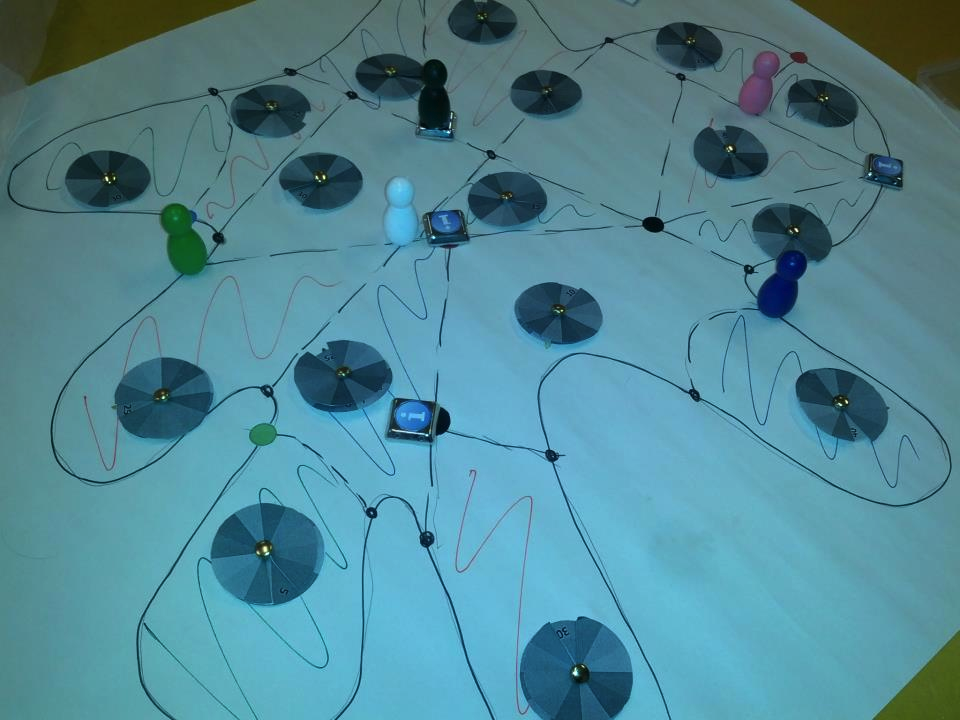
\includegraphics[width=1.0\textwidth]{img/paperprototype}
  \caption{Picture of the paper prototype} 
			% complete with colored zones, 
			% circular panic gauges, nodes, information centers, barricades 
			% and players 
  \label{fig:paperPrototype}
\end{figure}


\section{Constraints}

Only a few of us have some past experience with HTML5 and JavaScript\\
The game is to be completed within one semester (21 January - 27 May)

\section{Customer and supervisor}
The customer for this project is Ines Di Loreto, a researcher in the Department 
of Computer \& Information Science at NTNU. The supervisor assigned for this 
project is Mohsen Anvaari, a PhD candidate in the same department.




 \pagebreak
\chapter{Project Management}

\section{Process Model}
% TODO: Insert image
Due to the extensive need for documentation, Scrum is not a suitable model of 
this process. Moreover, the intended model of process cannot be fitted in a 
waterfall model. Therefore, the model used will be a mixture of the best 
properties from both models. First of all the architecture will be designed 
along with the production of a detailed, sensible documentation. Then a simple, 
“bare bone” version of the game will be developed. Finally, the required 
features will be iterated on this version.


\subsection{Kanban board}
% TODO: insert image 
The Kanban system fitted the project development process well, as a core 
prototype of the game was initially developed. Secondly, plans were made to 
add features such as a replay of a game session, an Expert interface and a 
database. It was decided to use an online version of a Kanban board called 
LeanKit Kanban. LeanKit was easy to use and enabled customizing the separation 
of tasks and processes on the board, as well as categorizing tasks by color. 
In addition, it enabled customizing the Kanban board, such as adding an extra 
“Testing” section for tasks.




\section{Roles and responsibilities (tentative)}
These are the roles assigned to the different team members:

\begin{itemize} \setlength{\itemsep}{0cm}\setlength{\parskip}{0cm}
	\item Customer/supervisor contact - Sindre Svendsrud
	\item Server manager - Jim Frode Hoff
	\item LaTeX configuration manager - Jim Frode Hoff
	\item Client manager - Stian Aurheim and Jørgen Foss Eri
	\item Expert interface manager - Adrian Arne Skogvold
	\item Team manager - Jørgen Foss Eri
	\item Test manager- Jens Even Berg Blomsøy
	\item Database manager - Jens Even Berg Blomsøy
	\item Documentation manager - Sindre Svendsrud
\end{itemize}
\\\newline
The LaTeX configuration manager was handed to Jim because he was the only one with prior experience to LaTeX. The rest of the roles were handed to the person who wanted that specific role. This was done because none of the group members had any more experience or knowledge about the roles than any of the others.
\\\newline

\noindent\textbf{Customer/supervisor contact}\\ % \noident == quickfix
The customer/supervisor contact is responsible for the communication with the 
customer and the supervisor. It is important that he shares important 
information such as time and place for meetings with the rest of the group.
\\\newline
\textbf{Server manager}\\
The server manager is responsible for the development of the server. That does 
not mean he has to do all the coding himself, but he has to make sure that 
everything that needs to be done on the server side is done. The main task is 
to implement the game rules.
\\\newline
\textbf{LaTeX configuration manager}\\
The responsibility of the latex configuration manager is to export the project 
report to latex and configuration of github.
\\\newline
\textbf{Client manager}\\
The client manager is responsible for the development of the client. That means 
that he has to make sure that the client is displayed correctly. Typical work 
here is the drawing of objects such as draw player or draw node. 
\\\newline
\textbf{Expert interface manager}\\
The expert interface manager is responsible for the expert interface. The 
expert interface sets up the game. The main task is to implement a way for the 
expert to set up the game.
\\\newline
\textbf{Team manager}\\
The team manager is responsible for the progress of the project. He makes sure 
deadlines are met, meetings are attended and that the team members are engaged.
\\\newline
\textbf{Test manager}\\
The test manager is responsible for writing the tests of the system. He should 
also make sure that the tests are performed.
\\\newline
\textbf{Database manager}\\
The database manager is responsible for the database, that means the design of the database (ER diagram) and the implementation of the database. Typical work here is to make database queries. 
\\\newline
\textbf{Documentation manager}\\
The documentation manager is responsible for the documentation of the project. The main tasks are to create and maintain the structure of the report.




\section{Time plan}
A time schedule to view planned tasks and their deadlines has been created in a 
Gantt chart (available as attachment). 
\\\newline
A short summary of the development can be seen as:\\
Version 1: Server game logic, client event handler, (simple) client view and 
communication module \\
Version 2: Addition of the administration interface and the expert client, 
extend view and game rule support\\
Version 3: Adaptation to other clients, extra features beyond the core \\

\subsection{Milestones} 
During the project there are certain milestones to be completed in time, both project report and technical milestones. \\
\newline
\textbf{Project report milestones}\\
10 February - Delivery - Project report: Preliminary version\\
15 March - Delivery - Project Report: Mid-semester version\\
19 April - Delivery - Project report: Final comments from supervisor\\
27 May - Delivery - Project report: Final version\\
\newline
\textbf{Technical milestones} \\
18 February - Barebone client that can communicate with the server \\
18 February - Barebone server that can communicate with the client\\
28 February - Basic prototype of the game\\
28 February - Database connection\\
11 March - Game v.1, a simple, working prototype of the game\\
22 March - Database queries\\
19 April - Expert interface for setting up the game\\
10 May - Game final\\
\newline
These are the code milestones which were set for the project in regards to the 
client/server/database functionality. The reason the milestones is in that 
order is because many of them depend on the milestones prior to them. \\


\section{Work breakdown structure}
% TODO: Legge inn bilde

\section{Risk list}
{\footnotesize
\begin{longtable}{| p{2.5cm} | p{1.5cm} | p{1.5cm} | p{1.5cm} | p{3cm} | p{3cm} |}\hline
	\textbf{Description} & \textbf{Likeli- hood} & \textbf{Impact (1-9)} & \textbf{Impor- tance} & \textbf{Preventive action} & \textbf{Remedialaction} \\
	\\\hline
	Data-loss (docs or code) 	& 3 & 7 & 21 
		& Continuous saving and version control. Distribute data among all group members. 
		& Try to retrieve data from computer/repository. Start from scratch, if necessary.
	\\\hline
	Network failure 			& 3 & 3 & 9  & 
		N/A & Switch to another network. Ask IDI for help, if necessary. 
	\\\hline
	Computer crash(es) & 4 & 7 & 28 & Continuous upload to repository & 
		Try to retrieve data. Worst case scenario: Retrieve most up-to-date data 
		from repository. Use computers from IDI (P15). 
	\\\hline
	Organization/ communication failure & 5 & 7 & 35  & Be watchful of correct 
		distribution of information. & Find out where communication failed and 
		restore the organization. 
	\\\hline
	Personnel absent due to sickness & 6 & 3 & 18 & Continuous upload to 
		repository. Be prepared to pitch in on others’ assignment, inform the 
		group that you are unable to meet on the day of sickness. \& Get update 
		and data from the person in question. Bring the person up-to-speed on 
		project, work done while he was away. & 
	\\\hline
	Great personal conflicts & 3 & 8 & 24 & Be prepared to withstand discussion 
		and criticism. Tell the other members of the group how you feel. Go to 
		the supervisor/ \& professor for advice if necessary. & Resolve the 
		issues with the help of a neutral part (supervisor/professor). 
	\\\hline
	Absent personnel & 7 & 3 & 21 & Point out the importance of attendance to 
		appointed hours. Inform ahead of time if leaving for vacation. See also 
		\emph{Personnel absent due to sickness}.  & Point out the importance of 
		attendance again. Notify student assistant if it becomes a problem. See 
		also \emph{Personnel absent due to sickness.}
	\\\hline
	Loss of personnel & 2 & 8 & 16 & Regular uploads of code and information 
		to repository & Notify supervisor of loss of personnel. Split work 
		assignments to personnel left in group.  
	\\\hline
	Incorrect system requirements & 3 & 8 & 24 & Be sure everyone has read and 
		understood the project requirements. Ask the customer if there any 
		uncertainties. & Resolve the incorrect requirements. Find out what went 
		wrong. Be confident that the other requirements are correct by 
		confirming with the customer.
	\\\hline
	Inexperienced with development technology & 8 & 3 & 24 & Be prepared to 
		search for information needed. Ask for help from supervisor if 
		necessary. Choose technology we are already comfortable with, if 
		possible. & Search and retrieve needed information. Get acquainted with 
		the technology needed. 
	\\\hline
	Misunderstand project & 2 & 9 & 18 & Make sure everyone has read and 
		understood the project goals, and that our goal(s) fit the customers 
		needs. Regular meetings with the customer for discussion regarding our 
		goals/customer needs. & Notify supervisor of grave errors/
		misunderstandings. Work out a rescue plan with the customer. 
	\\\hline
	Misunderstand subproblem & 2 & 8 & 16 & Make sure everyone involved has 
		read and understood the sub project problem/solution. & Correct the 
		mistakes and restart resolvement of subproblem. 
	\\\hline
	Error estimation of time needed & 5 & 5 & 25 & Be prepared for incorrect 
		time estimate, including error margins, avoid bursts. & Do bursts, 
		expand time schedules for work/work longer hours. 
	\\\hline
\caption{Risk assesment list}
\label{fig:risklist}
\end{longtable}
}


\section{Example of status report}
At the end of each week a status report will be sent to the customer and supervisor. This is an example of a status report that follows the given template: \\
\newline
Status report week 10 group 10\\
\\
\textbf{1 Introduction}\\
We now have a working prototype!\\
\\
\textbf{2 Progress summary}\\
The players can now move and de-panic zones, and turns are implemented. A timer for increased panic is implemented. The drawing functionality for objects works for the most part, and the database connection is now up and running. Css has been implemented for nice looks. Messages passing between the client and server (with json) work correctly.\\
\\
\textbf{3 Open / closed problems}\\
The database connection was a huge problem. It was detected that IDI had a firewall turned on. Much time was wasted due to error detection in the code (which was pretty much correct all the time).\\
\\
\textbf{4 Planned work for the next period}\\
Make database queries, event and information cards, roles and figure out how to implement effects (could be tricky). Produce documentation as always. Finish the requirements for the midterm report.\\
\\
\textbf{5 Updated risks analysis}\\
No updates needed.\\


\section{Communication}
During the project period it is important to continuously communicate with the customer. This way the customer is always informed on what has been done and enables giving feedback on what is desired next. In addition, the supervisor needs to be informed about the progress/work at all times. Finally, it is crucial that all team members communicate well.

\subsection{Interactions with the customer}
Regular meetings with the customer took place either weekly or bi-weekly. The meetings were scheduled through email. Prior to each meeting a presentation of the current state of the game was prepared. In addition, questions that needed answers regarding game functionality and rules were written. Simple logs of these meetings were kept to enable later reflections on the meetings. The fact that the customer is located at NTNU made it easy to set up schedules and have meetings.\\
\\
Throughout the meetings, the customer sometimes requested new tasks that went beyond the initial game functionalities. The was done because the customer was satisfied with the work so far, and wanted to provide extra challenges. These challenges were not required for this project, but if possible, they would add extra features to the game. An example of this was the possibility of using Sifteo Cubes as a game client, where the cubes would be used as zones. This was mentioned by the customer during one of the meetings. As this was not an important functionality, it was decided to focus 100\% on developing the JavaScript/HTML5 client, and perhaps test the Cubes at a later stage when the client was fully functional.



\begin{table}[H]
{\scriptsize
\begin{tabular}{|p{1.9cm}|p{1.9cm}|p{1.9cm}|p{3cm}|p{3.5cm}|p{3.5cm}|}
\hline
	\textbf{Date} & \textbf{Called by} & \textbf{Purpose} & \textbf{Preperation}
	 	& \textbf{Agenda} & \textbf{Notes} 
\\ \hline
	3/11/2013 & Customer & Update on where we are with the project
		& Implemented timer and cards (at least core functionality of cards), 
a task given to us on prior meeting 
		& Discussed how the amount of people should affect the panic level in 
the zones. Panic in a zone COULD be proportional to the amount of people, not 
important. Discussed events and how they could be solved by finishing a "quest" 
of different steps (example: if there is a fire: move people out, block zone, 
put out fire). These "quests" were not a requirement, only a suggestion. 
Discussed the use of Sifteo Cubes (an interactive game system with electronic 
gadgets) as a client, not a requirement. Important that we have a working 
game+client; other clients are "bonuses". 
		& This week we will work mostly with the report, not the game. This was explained to the customer.
\\\hline
\end{tabular}
}
\caption{Customer meeting log}
\label{fig:CustomerMeetingLog}
\end{table}

\normalsize


\subsection{Interactions with the supervisor}
The meetings with the supervisor took place bi-weekly and were scheduled through email. At these meetings the supervisor was informed about the work done since the last meeting. Problems and the group dynamic were also discussed. The supervisor provided feedback on the reports, which was much appreciated.

\subsection{Interactions within the group}
As there were meetings several times a week, much of the communication between the team members was done talking on a daily basis. In addition, meetings were planned and problems discussed through a facebook group. Facebook was chosen over e.g. email because all team members use facebook often, and long discussions through emails were regarded as messy.











 \pagebreak
\chapter{Prestudy}
\textbf{*} \emph{denotes the chosen alternative, if there were multiple choices.}

\section{Environment}
The first and probably most important decision to be made in this project was to decide on a language or software to serve as a development environment. There were several good alternatives, but finding one which was suited to both the task and accessible in terms of experience needed from the developers became a minor challenge.


\subsection{Front end language}
\textbf{Java}\\
The first and most obvious choice for any project on NTNU is Java, as it is the language used in most courses and all the team members are familiar with it. However, there are several issues when choosing Java for the front end. First of all, the ugly nature of the Swing framework is well known (although there are some alternatives). In addition, an applet in Java requires a plugin to work, if it is to be deployed on the web. A desktop version was an option, but that would limit the game to desktops only. Personal preference was also an issue with some of the developers, mostly regarding the Java’s static typing and rather verbose syntax.
\\ \newline
\textbf{Unity}\\
A program like Unity would lessen the amount of code on the client side, as creating a user interface and board for the game would be almost drag-and-drop, with some scripting to handle mouse interaction and data transfer with the server. However, in a boardgame that does not require more than 2D graphics, Unity would be overkill. It also requires a plug-in to work.
\\ \newline
\textbf{XNA}\\
This is a game development framework in C\# that runs on the xbox360 and windows platforms. Given that none of the team members were familiar with C\#, and the restrictiveness in terms of portability, this was not a good option.
\\ \newline
\textbf{HTML5 *}\\
The choice eventually fell on HTML5 as the best front end technology. With the proper browser, it runs on nearly all platforms, which was a key requirement for the game. Its simplicity in drawing 2D objects with the canvas element would be useful and make development faster. A couple of the team members were already familiar with HTML5 and JavaScript, which would present and manipulate the canvas. Furthermore, it would be useful for the whole team to increase the knowledge of JavaScript, as it is the most widespread programming language on the web.


\subsection{Back end language}
\textbf{Java}\\
Again Java presents itself as the most obvious option, as its use as a back-end language with the Spring framework is widespread. Personal preference was one of the decisive factors, as well as productivity. Compared to the alternatives, it seemed like this would be the most time-consuming option.
\\ \newline
\textbf{Python}\\
With web frameworks such as Django, Flask and others, Python was quickly named as a decent option. Most of the team members had some experience with the language and frameworks, and writing Python is quick (and fun, according to some). As an engine for a real time application though, it was considered unsuitable. 
\\ \newline
\textbf{Node.js / JavaScript *}\\
This platform was the most foreign to the team, yet it showed a lot of promise. First of all, the entire project could be written in one language, namely JavaScript, which would really hammer the concepts of prototyping (in JS) and give the team more experience with this popular language. Node is event-driven and relies heavily on asynchronous functions, which suited well with the imagination of producing an event-driven game. In the end, these factors made this option the best fit for making “Don’t Panic”.


\subsection{Data transfer protocol}
\textbf{JSON *}\\
Given that all the writing would be done in JavaScript, choosing JSON (JavaScript Object Notation) was easy. As JSON looks exactly like JavaScript objects, it was easier to understand and work with JSON than for example XML, which looks more like HTML and did not really suit the needs for a simple protocol to send commands and JS objects through.


\subsection{Database}
\textbf{MongoDB}\\
An analysis was made of MongoDB which actually stores the data in JSON documents instead of tables. This would be convenient, since it had already been decided to use JSON for data interchange. However none of the team members had any knowledge of MongoDB and it would be time consuming to learn it.
\\ \newline
\textbf{NoSQL}\\
NoSQL is efficient for storing a large amount of data that does not necessarily need to be structured. It does not offer any functionality beyond storage (like keys). It is faster than relational databases like MySQL. However there was no need for storing a large amount of data, and the data was structured. Therefore this was not a very good option.\\
\\ \newline
\textbf{MySQL*}\\
MySQL is the world’s most popular and used open source database. It is used by e.g. facebook, wikipedia and google. MySQL is a relational database management system and therefore fits well with the data. The team members had some experience with MySQL from earlier courses such as TDT4145 Data Modeling, Database and Database Management Systems and IT1901 Project 1. In addition the team knew that IDI could provide a MySQL database on their server, which was convenient. MongoDB seemed like a promising alternative, but this option was considered more time consuming than MySQL. That is why MySQL was chosen. 


\section{Frameworks}
\textbf{Socket.io *}\\
This is the go-to JavaScript library for real-time web applications using Websockets. It contains a client-side library that runs in the browser, and a server-side library for node.js. Like node.js, it is event-driven.
\\ \newline
\textbf{Node-mysql *}\\
This is a node driver for mysql. It enables connection to mysql database with JavaScript.
\\ \newline
\textbf{jQuery *}\\
The jQuery library simplifies access to the DOM, provides animations and easy element content manipulation.
\\ \newline
\textbf{Express *}\\
This is a web development framework for node.js, that simplifies access to routing, requests and sessions. 


\section{Versioning}
\textbf{Subversion}\\
This is often the standard versioning system used at NTNU, as a repository is provided by IDI, and the team members have used it in several courses already. It is a centralised system and more mature in its development than Git, the alternative. However, it is slow in comparison. Branching is cumbersome and if the central server is not available, it can cause significant trouble.
\\ \newline
\textbf{Git  *}\\
In Git, all clones of the repository act as a back up, and the system itself is distributed, where a clone on Github (in this case) acts as a communication channel between the users. Some of the team members already had experience using Git, and found it a lot easier and faster to setup and use in practice.


\section{Project management tools and processes}
\textbf{Google Drive}\\
Google Drive is a file storage and synchronization service provided by Google that enables collaborative editing of the project documentation. For this project documentation Google docs was used. As this is a collaboration based tool, it suited the structure of the work method. 
\\ \newline
\textbf{Dia}\\
In addition to the documentation tools for diagrams provided by Google Drive a program for creating various diagrams, Dia was used. This program has templates of almost all UML designs. 
\\ \newline
\textbf{Wbstool}\\
Wbstool was used to make the work breakdown structure chart. 
\\ \newline
\textbf{Kanban}\\
Kanban is a method for developing software with an emphasis on just-in-time delivery, while making certain not to overload the developers of the system with work. At the heart of Kanban lies the Kanban board; a visual process management tool consisting of a Kanban board and cards. Each card represents a task that can be assigned to members of the development team. The board is divided into sections, separating tasks that have only been defined, from tasks that are in progress and tasks that are finished. Using this system, any member of the group can create and assign tasks to other group members, and keep an eye out for who is doing what at any given time.


\section{Existing solutions}
Since this is an original board game developed by the customer, there are no alternative electronic solutions of this game already developed. However, there is a large number of other board games that have been adapted into a digital version using various technologies.\\

Examples:\\
- Chess: http://plainchess.timwoelfle.de/\\
PlainChess is a chess implementation built completely using HTML5 technologies. The game engine is written in JavaScript and relies on the frameworks jQuery and jQuery UI, and games can be played both with and without the use of an internet connection.\\

- Planet Sudoku: http://planetsudoku.com/\\
Planet Sudoku is a robust, customizable HTML5 Sudoku game supporting different kinds of Sudoku rules and difficulty settings.\\

- Bombermine: http://bombermine.com\\
Bombermine is a massively multiplayer online adaption of the classic strategic puzzle game Bomberman by Hudson Soft/Konami. The game was made with HTML5 and JavaScript, using the AngularJS and async.js frameworks. Bombermine won the Best Web-Only Game at the Mozilla Game On 2013 competition, and although it is not as similar to a traditional board game like Don’t Panic is, it really shows the possibilities for HTML5/JavaScript games.\\

After having reviewed these example games, it was clear that the chosen technology of HTML5 and JavaScript was a good choice for creating the game.\\

 \pagebreak
\chapter{Requirements}
\section{Functional requirements}


FR1 - Expert Interface\\
A crisis management expert should be able to set up a game template for teams to use. This interface should be able to configure as many variables in the game as possible(game rules), and be able to create maps, change the number of players, where they start, what events can occur and when, and create information cards.\\
\\
FR2 - Game Manager\\
An expert should be able to enter an existing game as a Game Manager. The GM should be able to trigger events and modify the game objects on the fly to make the game more dynamic, as well as comment on player actions. The GM should be able to monitor activity on the server, existing sessions and online players.\\
\\
FR3 - Player Profiles\\
Each player should have a profile that records the players performance in played games. This includes tracking wins and losses, listing game replays and other metrics that are relevant.\\
\\
FR4 - Replay\\
An expert should be able to view finished games as a re-play, to evaluate player performance. These replays should be stored in , to be viewed at any time.\\
\\
FR5 - Game functionality\\
In addition to adapting the functionality of the board game version to an electronic platform, as specified in the appendix, the number of people in a zone should affect how panic spreads between zones, and inside them. \\
\\
FR6 - Physical interaction\\
Preferably, the game should be able to respond to commands sent by interaction devices such as Arduino or Sifteo cubes. They could be used to represent zones, players or be used as controllers for movement.\\
\\


\subsection{Use cases}
The use cases are mainly based on the functional requirements of the game and are a graphical representation of the users’ interactions with the board game. They document all the different ways in which the user can interact with the game. 
\\
A detailed set of use case diagrams and textual use cases are provided below.\\


% START USE-CASE TABLES
\begin{table}[H]
\begin{tabular}{|l|l|} \hline
	\textbf{ID} & \textbf{01}\\ \hline
	Name & Login Player\\ \hline
	Goal & To be connected to the server\\ \hline
	Actors & Player, server\\ \hline
	Start requirements & None\\ \hline
	End requirements & - The player gets logged in.\\
					 & - The game is displayed.\\ \hline
	Case & - The player clicks on the option for player, in the middle of the HTML starpage\\
			& - The player gets prompted with the login form. \\
		 	& - The player gives login-info.\\
			& - The player clicks the login button to the rigth of the form.\\
			& - The player is now logged in.\\ 
			& - The player is moved to the player's page. \\ \hline
	Alternative Case & Wrong password\\ \hline
	Previous Use Case & None\\ \hline
	Spawned Use Case & 05\\ \hline
\end{tabular}
\caption{Use Case: Login player}
\label{fig:usecase01table}
\end{table}


\begin{table}[H]
\begin{tabular}{|l|l|} \hline
	\textbf{ID} & \textbf{02}\\ \hline
	Name & Login Expert\\ \hline
	Goal & To be connected to the server\\ \hline
	Actors & Expert, server\\ \hline
	Start requirements & None\\ \hline
	End requirements & - The expert gets logged in.\\
					 & - The expert view is displayed.\\ \hline
	Case & -The expert clicks on the option for expert, in the middle of the HTML starpage\\
			& - The expert gets prompted with the login form. \\
		 	& - The expert gives login-info.\\
			& - The expert clicks the login button to the rigth of the form.\\
			& - The expert is now logged in.\\ 
			& - The expert is moved to the expert's page. \\ \hline
	Alternative Case & Wrong password\\ \hline
	Previous Use Case & None\\ \hline
	Spawned Use Case & 03\\ \hline
\end{tabular}
\caption{Use Case: Login expert}
\label{fig:usecase02table}
\end{table}

\begin{table}[H]
\begin{tabular}{|l|l|} \hline
	\textbf{ID} & \textbf{03}\\ \hline
	Name & Game Setup\\ \hline
	Goal & To create a successful game session\\ \hline
	Actors & Expert, server\\ \hline
	Start requirements & The expert is logged in\\ \hline
	End requirements & The expert is able to create a game setup \\ 
						& The expert is able to save the game setup\\ \hline
	Case & The expert creates the appropriate map for the game. By ploting nodes into the canvas and creates paths between them. To create a zone the expert selects a minimun of 3 paths and clicks for create zone.\\
			&- The expert adds the wanted board pieces by clicking on the corresponding buttons for the different game pieces, while in the wanted node. \\
			&- The expert selects what type of zone the selected zone should be, and does this for each zone.\\
			&- The expert set the number of people for each zone, by selecting a zone and using the initial people button at the top of the canvas.\\
			&- The expert sets the initial panic for each zone by selecting the zone and the corresponding button for initial panic, at the top of the canvas.
			&- The expert manages the cards, there is an initial set of cards for the game, but if the expert wants he can add more, or special cards at the top of the page, over the canvas for drawing the map.\\
			&- The expert adds the wanted number of players to the game, by selecting a node and by using the add player button.\\
			&- The expert can set a individual starting point to each player by selecting the wanted node and by using the button for add player at the top of the canvas.\\
			&- The expert assigns roles to each player, by selecting a player from the form over the canvas for creating the map. \\
			 \hline
	Alternative Case & None \\ \hline
	Previous Use Case & 02\\ \hline
	Spawned Use Case & 04, 05\\ \hline
\end{tabular}
\caption{Use Case: Game Setup}
\label{fig:usecase03table}
\end{table}

\begin{table}[H]
\begin{tabular}{|l|l|}
\hline
	\textbf{ID} & \textbf{04}\\ \hline
	Name & Watcher\\ \hline
	Goal & To get a non player version of the game\\ \hline
	Actors & Expert, server\\ \hline
	Start requirements & The expert is logged in, a game is running \\ \hline
	End requirements & The expert is able to watch the wanted game\\ \hline
	Case &- From the monitor game option at the top of the expert page, the expert gets a list of games in session, the expert selects one of these to start monitoring the game.\\
		 &- The server provides a game window in which the expert is not participating as a player\\ \hline
	Alternative Case & None \\ \hline
	Previous Use Case & 02\\ \hline
	Spawned Use Case & None\\ \hline
\end{tabular}
\caption{Use Case: Watcher}
\label{fig:usecase04table}
\end{table}

\begin{table}[H]
\begin{tabular}{|l|l|}
\hline
	\textbf{ID} & \textbf{05}\\ \hline
	Name & Join Game\\ \hline
	Goal & To successfully join a starting game\\ \hline
	Actors & User, game session, server \\ \hline
	Start requirements & A game has been created by the exper\\ \hline
	End requirements & A user is able to join the appropriate game\\ \hline
	Case & The user clicks on join options for the game in the middle of the page\\
			&- The game asks for user info in a popup form, the user enters the info. \\
			&- The user joins the game \\ \hline
	Alternative Case & The user gives incorrect info and is not added to the game \\ \hline
	Previous Use Case & 03 \\ \hline
	Spawned Use Case & 06, 07\\ \hline
\end{tabular}
\caption{Use Case: Join Game}
\label{fig:usecase05table}
\end{table}



\begin{table}[H]
\begin{tabular}{|l|l|}
\hline
	\textbf{ID} & \textbf{06}\\ \hline
	Name & Move game pieces \\ \hline
	Goal & To move a game piece to a wanted location \\ \hline
	Actors & Player, game board, game session, server \\ \hline
	Start requirements & The player has joined a game \\
				& The player in question has the turn \\ \hline
	End requirements & The player is able to move the selected piece to the wanted position. \\ \hline
	Case &- The player uses the mouse pad to select the wanted object. \\
		&- The player drags the object through the path to the wanted location. \\
		&- The game board is updated. \\ \hline
	Alternative Case & The player selects an immovable object \\
				& The player moves the object to an unobtainable location\\ \hline
	Previous Use Case & 06 \\ \hline
	Spawned Use Case & None\\ \hline
\end{tabular}
\caption{Use Case: Move game pieces}
\label{fig:usecase06table}
\end{table}

\begin{table}[H]
\begin{tabular}{|l|l|}
\hline
	\textbf{ID} & \textbf{07}\\ \hline
	Name & Use information cards\\ \hline
	Goal & To use an information card to affect the board\\ \hline
	Actors & Player, Game Board, Game Session, Server\\ \hline
	Start requirements & The expert has created a game\\
				& The player is logged in\\
				& The player is part of a game\\
				& The player has an information card \\ \hline
	End requirements & The card effect is carried out on the board\\
				& The player does not have the used information card \\ \hline
	Case & The player clicks on the wanted information card under his player profile to the side of tha canvas.\\
		&- The information card effect is carried out on the board\\
		&- The player loses his information card \\ \hline
	Alternative Case & None \\ \hline
	Previous Use Case & 05\\ \hline
	Spawned Use Case & None\\ \hline
\end{tabular}
\caption{Use Case: Use information cards}
\label{fig:usecase07table}
\end{table}


\begin{table}[H]
\begin{tabular}{|l|l|}
\hline
	\textbf{ID} & \textbf{08}\\ \hline
	Name & Use player action \\ \hline
	Goal & The player uses an action and the game board is updated\\ \hline
	Actors & Player, Game Board, Game Session, Server \\ \hline
	Start requirements & The user is logged in \\
				& The user is a player in the game\\
				& A game is in action\\ \hline
	End requirements & The player uses an action \\
				& The effect is updated on the board \\ \hline
	Case &- The player selects a adjacent node or a zone with the mouse pad.\\
		&- The player selects an action wich will appear at the top of the canvas after selecting a node or zone.\\
		&- The action is used on the target.\\
		&- The game board is updated.\\ \hline
	Alternative Case & None\\ \hline
	Previous Use Case & 05\\ \hline
	Spawned Use Case & None\\ \hline
\end{tabular}
\caption{Use Case: Login expert}
\label{fig:usecase08table}
\end{table}
% END USE-CASE TABLES



\section{Non functional requirements} 


All non functional requirements comply with the definitions as stated in the ISO 25010 standard (replacing ISO 9126). Only relevant requirements are mentioned in this report.

\subsection{Quality in use}

\emph{1: Efficiency}\\
Like regular board games, actions should not be difficult to execute. The players are working against the clock (the panic increase timer). Hence, when designing the user interface, one of the aims should be to minimize the number of clicks required.
\\\newline
\emph{2: Context Coverage}\\
The system should be flexible enough to accommodate individual experts’ preferences and needs in their simulations. By relying on the settings given by the expert through the expert interface form, the best possible flexibility can be ensured.

\subsection{Product quality}

\emph{1: Functional suitability}\\
Functional completeness should be achieved to include the core functionality 
of the board game, as well as the functionality specific to the electronic 
version, like the expert interface and panic- and people management. 
\\
Core functions must be without game-breaking bugs to ensure functional 
correctness.
\\\newline
\emph{2: Operability}\\
Usability is considered important, as the users should spend time playing the 
game and learn how to manage panic, rather than how to operate the game. 
\\
By exploiting recognisability from classic board games, a lot of interaction 
can be made intuitive, given that most people already know how to play board 
games. 
\\
Users of the game will most likely not be as proficient with computers as 
“gamers” in general. Therefore, it would be a good idea to make the game 
accessible without having to install any software other than an internet browser.
\\\newline
\emph{3: Transferability}\\
The client should be usable on as many platforms as possible (Mac, Windows, 
Linux, Mobile platforms), and in the best possible case be able to interact 
with devices such as Arduino. HTML5 with node.js was chosen for this reason, as 
it can run on nearly any device without the need for time consuming 
installation procedures, thereby increasing portability.


\subsection{Technical requirements}
These requirements have been copied from the “Don’t Panic” specifications 
provided by the customer.\\

Don’t Panic DPS has to meet to the following requirements:\\
- All interaction between the server and client SHOULD be performed using well 
documented protocols and standard protocols.\\
- The DPS Game rules SHOULD be platform independent. Consequently, high level 
languages such as Java, Processing, Python COULD be considered as good 
candidates.\\
- The overall architecture SHOULD be scalable to run multiple Game sessions in 
parallel without decreasing the quality of already running games sessions.\\
-Already existing frameworks for game development for such as Unity, Microsoft 
XNA Game Studio, or management tools such as RedMine COULD be used as platforms 
to help speeding up the development of the game. The choice should be driven by 
a framework comparison analysis considering both technical requirements and 
already existing skills/experience among group participants.






 \pagebreak
\chapter{Design and architecture}

\section{User interface}

\begin{figure}[H]
  \centering
    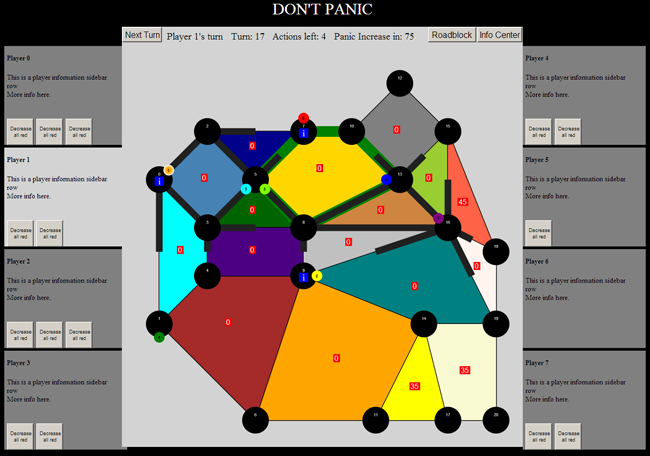
\includegraphics[width=1.0\textwidth]{img/earlyVersion.png}
  \caption{User interface, ' The user interface of the game, complete with a board, pieces, cards and information tables'} 
  \label{fig:earlyversion}
\end{figure}









\subsection{User interface design}

The customer had already designed a physical board game of Don’t Panic, which formed the basis for designing the electronic version. In the earliest stages of the designing Balsamiq Mockups was used, an online tool for interface designing.\\
\\
Mockups is designed to be an easy and efficient tool used in the early stages of interface designing, and it can be used to generate click-through prototypes for interfaces. Through myBalsamiq it can also be used as a collaborative tool, supporting project-based collaboration and real-time changes.\\

\begin{figure}[H]
  \centering
    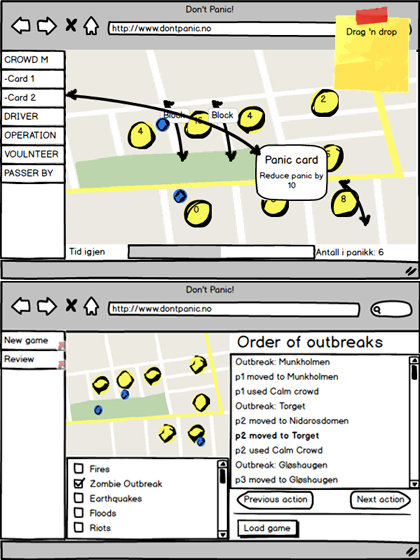
\includegraphics[width=1.0\textwidth]{img/mockups.png}
  \caption{User interface, ' Early design of the board, cards and the expert interface'} 
  \label{fig:mockups}
\end{figure}




\subsection{Realisation of the user interface}

\begin{figure}[H]
  \centering
    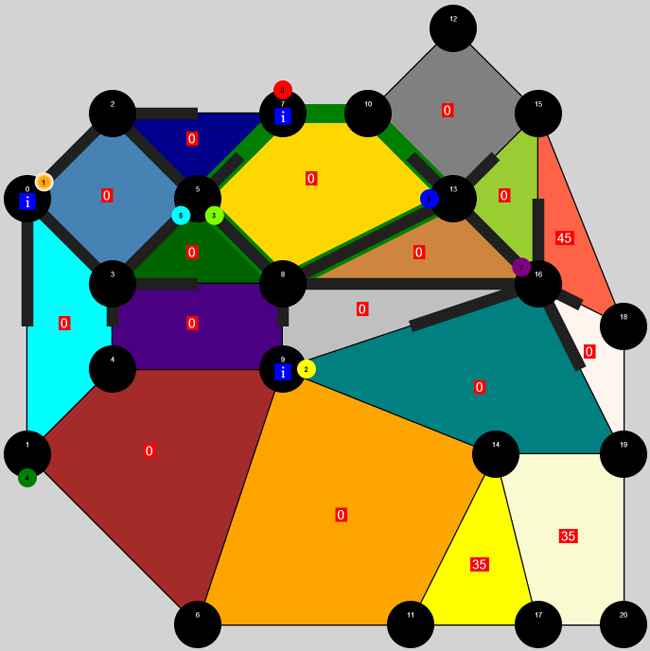
\includegraphics[width=1.0\textwidth]{img/canvas.png}
  \caption{User interface, 'The canvas'} 
  \label{fig:canvas}
\end{figure}


The main part of the interface is the HTML5 canvas. The board and pieces of the game are all drawn within this canvas using JavaScript. The players are able to control their respective player pieces by dragging them on the board from one node to another using the mouse, like one would do using the hands when playing the physical version of the board game. One of the main goals of the project was to preserve the physical interaction of playing a board game in the electronic version, so it was decided that implementing a drag-and-drop functionality for the player pieces would be a good idea. \\
\\
The panic levels for each zone are printed inside the zones. This was very cumbersome with the physical version, as the players were forced to update all the zones manually each time the timer counted down, as well as when event cards and information affected the zones. This is now handled automatically on the server. \\


\begin{figure}[H]
  \centering
    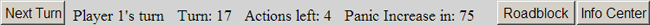
\includegraphics[width=1.0\textwidth]{img/headtable.png}
  \caption{User interface, 'The head table'} 
  \label{fig:headtable}
\end{figure}

An information table is placed above the canvas. This table contains the button the players would use when ending their turns, as well as buttons for placing information centers and roadblocks on the nodes they are located. The table also contains information about whose turn it is, how many turns have passed, how many actions the active player has left and a timer which counts down to the next increase in panic. \\
\\
On each side of the canvas there are sidebar rows. Players have their own row, which is highlighted when it is their turn. The rows contain information on players, as well as their information cards. Since this is a collaborative game, all the cards should be visible to the players so they can openly discuss how the cards should be used, as well as trade cards between themselves. This preserves the verbal interaction dynamics of a physical board game. The cards are implemented as buttons with text corresponding to their effect in the game. \\

\begin{figure}[H]
  \centering
    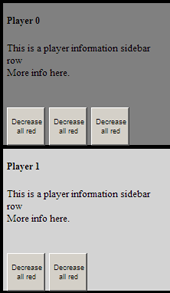
\includegraphics[width=0.4\textwidth]{img/sidebarrowssmall.png}
  \caption{User interface, 'Sidebar rows'} 
  \label{fig:sidebar}
\end{figure}




\section{Client/Server architecture}
A client-server model was chosen as the architectural pattern. This was highly desired by the customer, as they wanted different clients
to work with the server. Therefore using a different architecture was never considered as an option.

\subsection{Initial suggestion for a high level architecture from the customer}

\begin{figure}[H]
  \centering
    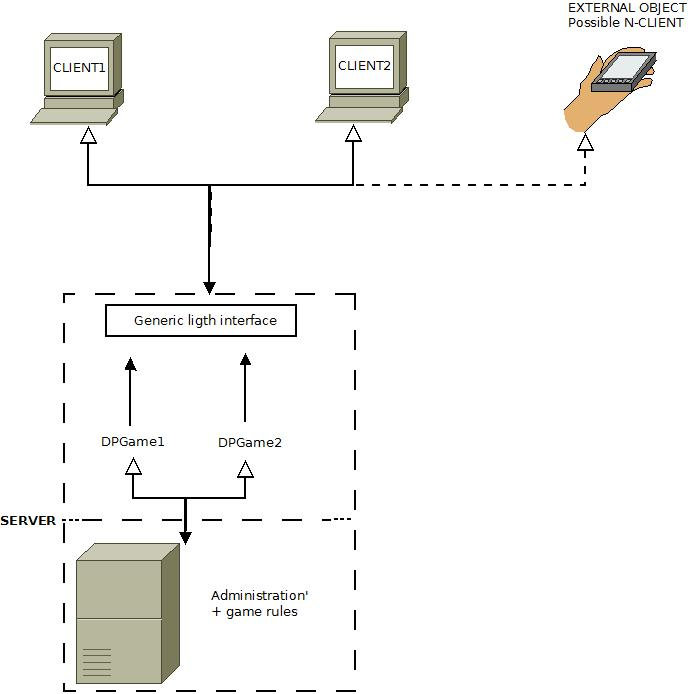
\includegraphics[width=1.0\textwidth]{img/Client-serverarchitecture.jpeg}
  \caption{System architecture, 'Initial suggestion'} 
  \label{fig:initialsuggestion}
\end{figure}



\subsection{High level system architecture}

\begin{figure}[H]
  \centering
    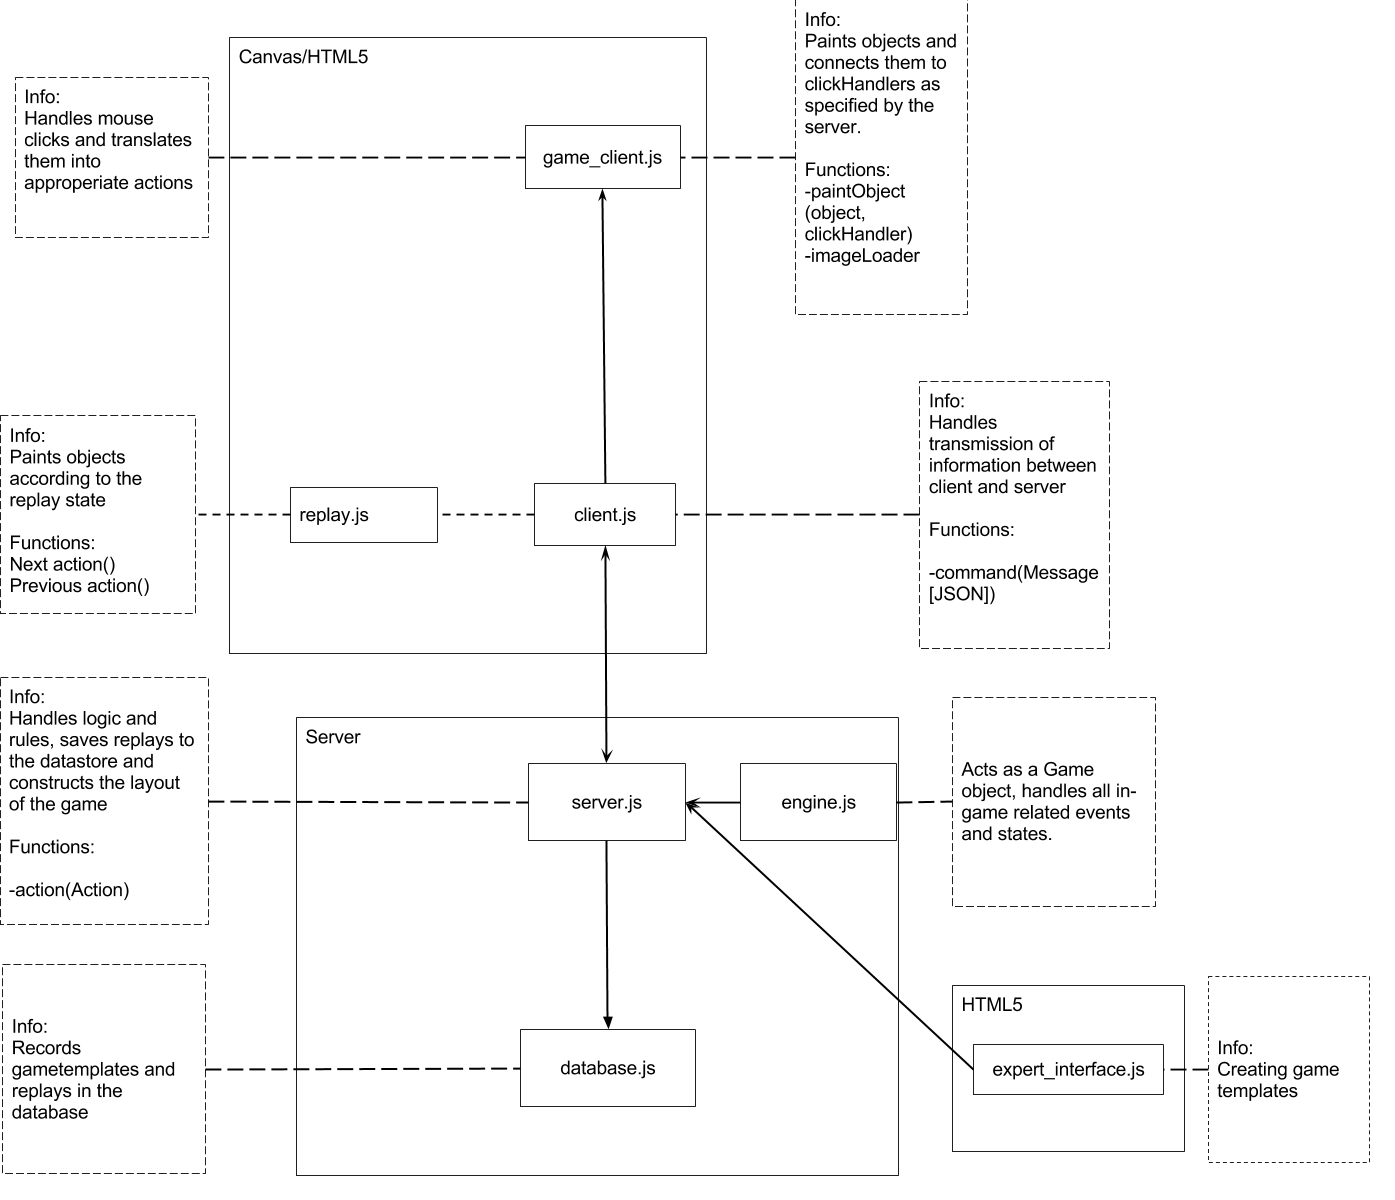
\includegraphics[width=1.0\textwidth]{img/highlevelarch.png}
  \caption{System architecture, 'High level system architecture'} 
  \label{fig:highsysarch}
\end{figure}

\subsection{Object diagram}

\begin{figure}[H]
  \centering
    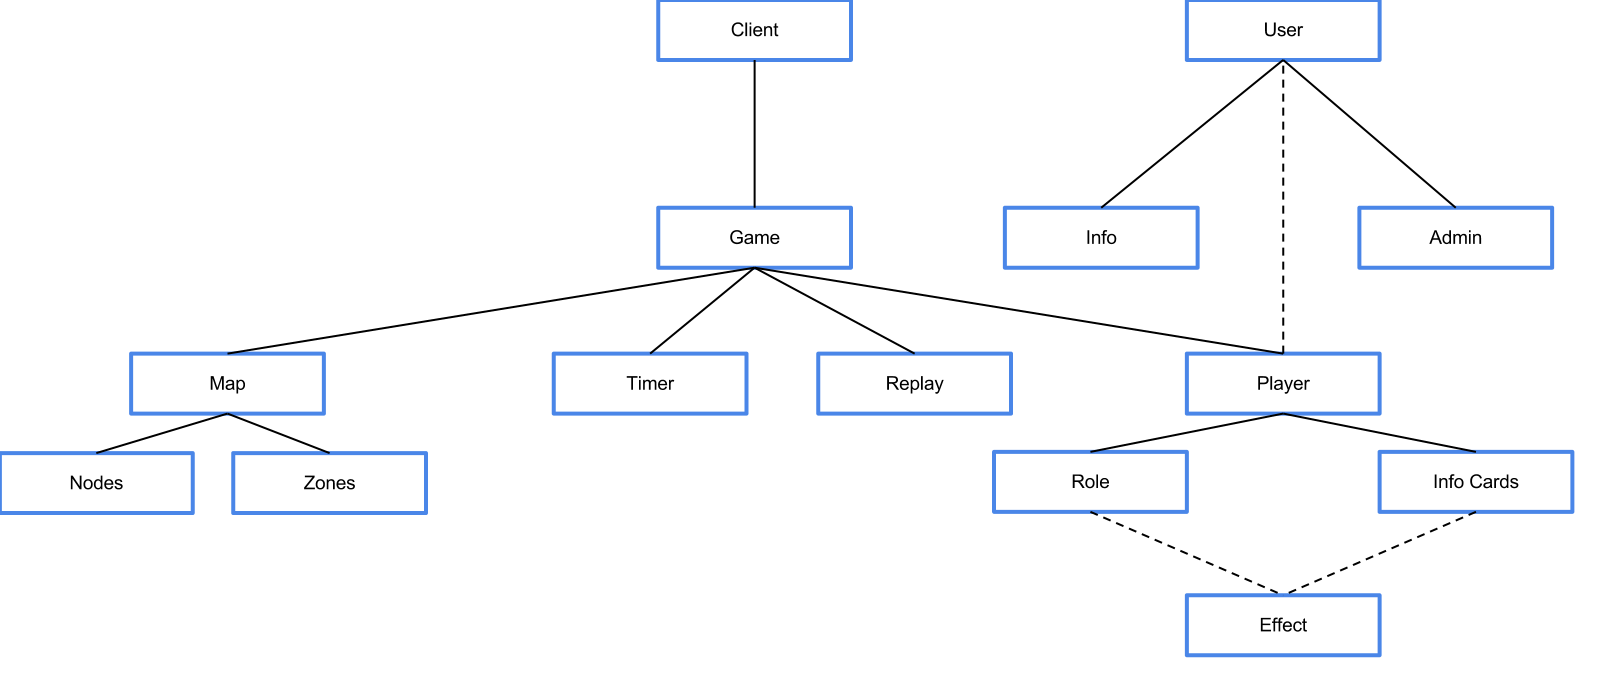
\includegraphics[width=1.0\textwidth]{img/GameTree.png}
  \caption{Object diagram, 'Game tree'} 
  \label{fig:gametree}
\end{figure}


\subsection{ER diagram}
\begin{figure}[H]
  \centering
    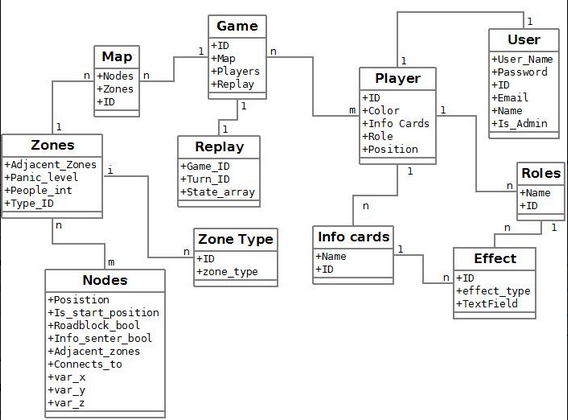
\includegraphics[width=1.0\textwidth]{img/erdiagram.png}
  \caption{'ER diagram'} 
  \label{fig:erdiagram}
\end{figure}

\subsection{Object hierarchy}
This chart is intended to show a high level view of the hierarchy, and how the objects are connected together to avoid loops. 

\subsection{Sequence diagrams}

The sequence diagrams show the interactions between the files, functions and methods. It depicts the objects and files interactions in the right time sequence. The diagrams also show the calls each method or a file sends to the next file, function or method.  \\


\begin{figure}[H]
  \centering
    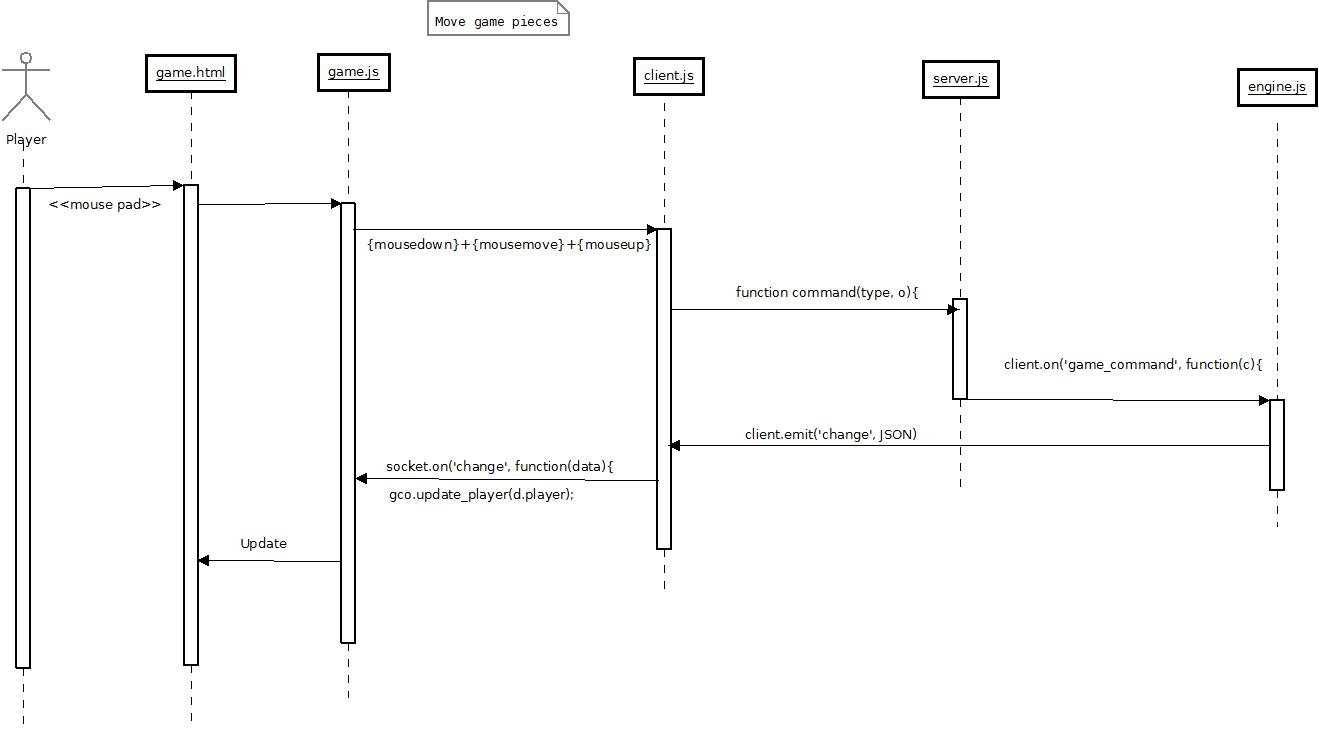
\includegraphics[width=1.0\textwidth]{img/movegamepiececsekvensdiagram.jpeg}
  \caption{Sequence diagram, 'Move game piecec'} 
  \label{fig:movegamepieceseq}
\end{figure}

The above diagram show the interaction between the JavaScript  files when a player decides to move his or hers game piece. The player initializes the sequence by clicking on the game piece in his HTML view. The first file after the HTML view is the game.js, the file that handles and interprets player inputs. The game.js file interacts with client.js which is the file handling every visual update of the game board. The file server.js Imports http and makes a server that socket.io can listen to; it connects the game interactions and game view with the engine. The file engine.js handles the game logic and game rules. When the interaction is at this point the engine.js fires a change to the client that in turn updates the view in the HTML file.\\


\begin{figure}[H]
  \centering
    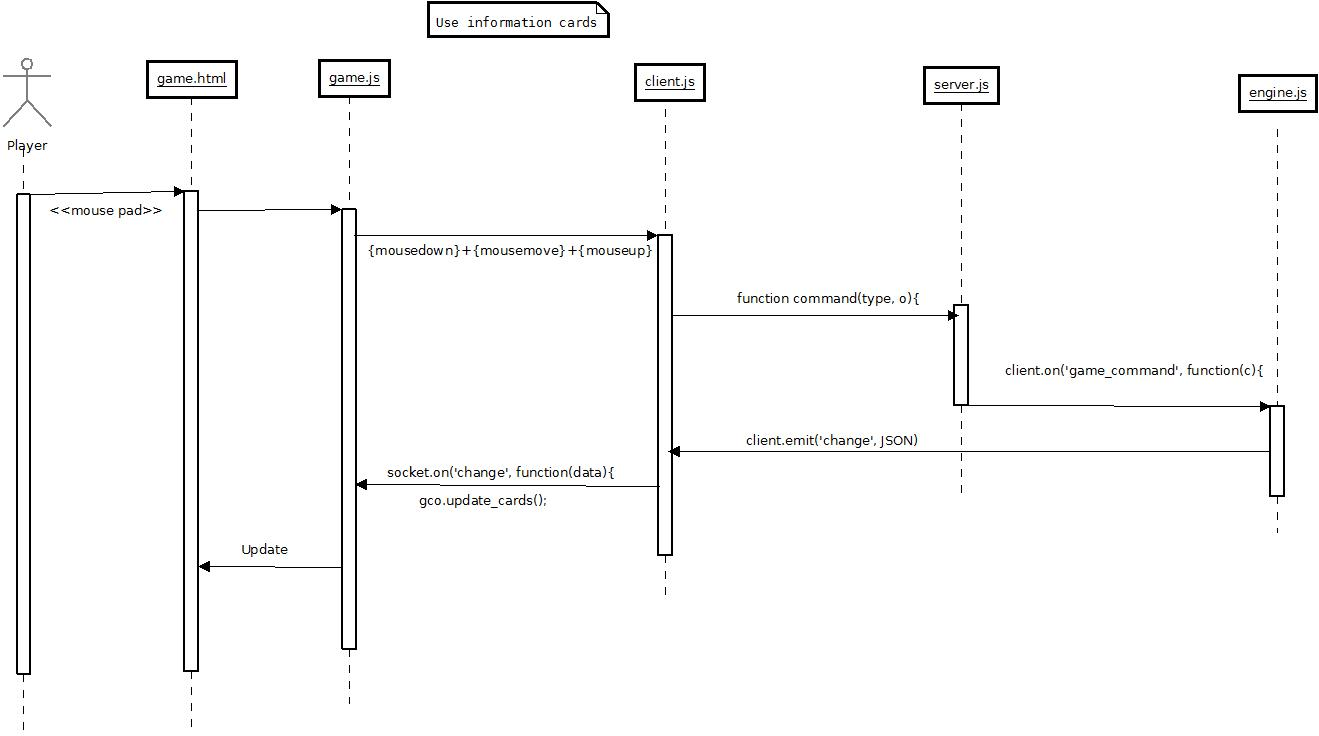
\includegraphics[width=1.0\textwidth]{img/useinfocardssekvens.jpeg}
  \caption{Sequence diagram, 'Use information card'} 
  \label{fig:useinfoseq}
\end{figure}

The above diagram shows the interactions of the JavaScript files when a player uses an information card in the game. The sequence is very similar to the previous diagram but is different in the types of data or methods it sends between the files. At the end it updates different parts of the game (gco.update();).\\


\begin{figure}[H]
  \centering
    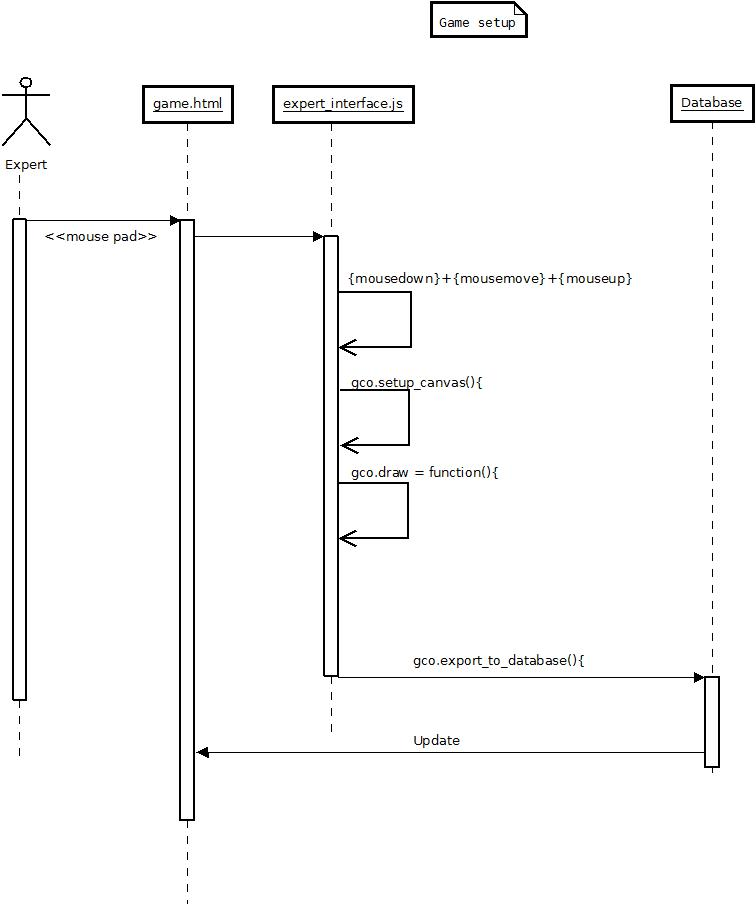
\includegraphics[width=1.0\textwidth]{img/gamesetupsekvens.jpeg}
  \caption{Sequence diagram, 'Game setup'} 
  \label{fig:gamesetupseq}
\end{figure}

The above diagram shows the interaction of the JavaScript files when an expert creates a game, the details of this is explained thoroughly in the use cases. The expert uses the mouse pad to interact with the game.html page, and is directed to the expert interface. The file expert interface.js is where all the dragging of the nodes, and creating and placing of the zones and players are created. When the expert is finished the game object is stored to the database. The last interactions is when game.html is updated when it get notifications from the database. The game can now be chosen from a list in game.html and played. \\

 \pagebreak
\chapter{Testing}
\section{Test plan}
The game will be tested thoroughly by both Black Box and White Box testing. Black Box testing will be the main point in this test plan. White Box testing will be done throughout the project and continuously, while the code is being written. An analysis was made of the pros and cons of writing small automated tests for the game, and the conclusion was that this would be more work for not enough profit. When the core of the game is finished the game development process switches from intertwined code to adding rules and actions to the game. This can be seen as layers. When the layering on top of the game core is done, it is not that difficult to test the added methods by itself. For this reason automated tests will not be written.\\
\\
For the Black Box testing a series of tests will be written, based upon the requirements specified in Chapter 2: Requirements. The Black Box testing implies thorough interaction between the team and the game. The aim is to see how the different objects on the map interact with each other, to find incorrections and glitches. In addition to testing the game for errors usability tests will be gone through. The usability tests will be done with an external actor to ensure independent feedback.The testperson will go through the different use cases to ensure satisfiability. \\

\subsection{Black Box testing}

The Black Box testing will shadow every part of the game. It is important that every part of the game is as error free and glitch free as possible. These are the test areas which will be looked closely at:

\begin{itemize} \setlength{\itemsep}{0cm}\setlength{\parskip}{0cm}
	\item The start of the game, such as login and menus
	\item The art of the game. These include the board model, player models and other object models contained in the game
	\item The movements of the game, moving board pieces around and the use of information cards 
	\item The view of the game board, borders and accurate frames
	\item The game flow, how the board game reacts to different turns
	\item The events and triggers within the game
	\item The interaction of the gamepad within the game
	\item The game rules (the tester needs to be familiar with the rules)
	\item A test for objects overlapping within the game, clipping
	\item Testing for multiplayer version, running more than one game, and as many as possible at one point
	\item Testing memory overload by leaving it on for an extended period of time. This is one of the few negative testing features that the game will go through
	\item A test for platform compatibility, since this is HTML5 based the platform will be different web browsers
\end{itemize}
\noindent
After testing has been done thoroughly, the testing phase will go on to tests with people unattached to the project. Unattached people will be used because it will be helpful to get feedback from someone outside the group. If there is something missing or incomprehensible, it provides the opportunity to correct or improve the error. The test person will go through the test provided, based on the use cases from the requirements. Common formalities such as voluntariness, choices and uncomforts will be gone through before the tests are made.\\
\\
Some points that will be confined to are:

\begin{itemize} \setlength{\itemsep}{0cm}\setlength{\parskip}{0cm}
	\item Under the tests the tester will not receive any help (unless unforeseen events occur that requires it).
	\item The tester has the choice to abort the tests at any moment
	\item The tester should think aloud, so that the choices made will be easier to understand
	\item The supervisors (the team) should take notes 
	\begin{itemize} \setlength{\itemsep}{0cm}\setlength{\parskip}{0cm}
		\item of problems during the tests.
		\item when the tester is unsure about what to do.
		\item when the tester does something wrong.
		\item if the tester does not know what to do at all.
		\item of any unforeseen events that occur during the tests.
	\end{itemize}
\end{itemize}
\noindent
After the tests are done a SUS sheet will be provided for the tester where he can evaluate the different parts of the system. Here is also the time for discussion and inputs from the tester. The supervisors have at this point taken several notes, and will have some questions about some of them to ask the tester.\\
\\
The result from each test and the comments will be shown in the tables below. Each table will provide:\\
\begin{itemize} \setlength{\itemsep}{0cm}\setlength{\parskip}{0cm}
	\item Test number
	\item Test case
	\item Comments about the test
	\item Problems during the tests and comments of these
	\item Proposals for solutions
	\item Improvements absolutely needed
	\item Small tweaks wanted
\end{itemize}


\subsection{System usability testing}
The tester is provided with the SUS (System Usability Score) sheet. The SUS sheet is a questionnaire containing 10 statements. The tester is expected to respond to each statement by choosing one of five options, depending on the degree of agreeability.\\
\\
The statements are:
\begin{enumerate} \setlength{\itemsep}{0cm}\setlength{\parskip}{0cm}
	\item I think that I would like to use this system frequently.
	\item I found the system unnecessarily complex.
	\item I thought the system was easy to use.
	\item I think that I would need the support of a technical person to be able to use this system.
	\item I found the various functions in this system were well integrated.
	\item I thought there was too much inconsistency in this system.
	\item I imagine that most people would learn to use this system very quickly.
	\item I found the system very cumbersome to use.
	\item I felt very confident using the system.
	\item I needed to learn a lot of things before I could get going with this system.
\end{enumerate}
These are the 5 choices:

\begin{figure}[H]
  \centering
    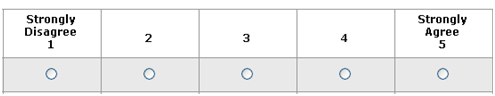
\includegraphics[width=1.0\textwidth]{img/sus-responses.png}
  \caption{Testing, 'SUS choices'} 
  \label{fig:paperPrototype}
\end{figure}






\subsection{White Box}

For the white box testing we have done small tests locally without pushing it to git. We have tried to keep one branch on our git repository free from errors, and only pushing working and error free versions of the game. The white box testing process has been an continuously task throughout the game development. The line "console.log('error');" has of course been of great help. The testing we have done of white box  has not been documented, as we found nothing of importance to document when we decided to not use unit tests. Since this is a smaller project, members of the group has had widespread and deep knowledge of the complete source code, and therefore white box testing has been possible.


\subsection{Tests}

\subsection\subsection{Black Box tests}
%%%%%%%%%%%%%%%%%%%%%%%%%%%%%%%%%%%%%%%%
% 1


{\footnotesize
\begin{table}[H]
\begin{tabular}{| p{5cm} | p{10cm} |}\hline
	\textbf{ID}	& \textbf{01}\\ \hline
	Name		& Game Start\\ \hline
	Time schedule	& Approximately 10 minutes \\ \hline
	Enviorment requirements 
		& The test computer must have internet access. \\
		& Regarding software, only a web browser is required. \\ \hline
	Test risk analasys 
		& Connection failure - Plausible \\ 
		& \emph{* Try to connect again. If the error persists, use another computer.} \\
		& \emph{* If switching computer does not resolve the connection failure, use another network.}\\ \hline
	Goal	& The test is to verify that the player can log in and start a game without problems. \\ \hline
	Actors	& Player, Game Board, \emph{Game Session, Server}\\ \hline
	Test requirements
		& The player can connect with the server. \\
		& The player can not log in with incorrect credentials. \\
		& The player can join the selected game. \\
		& The player cannot join an unintended game.\\ \hline
	End requirements 
		& The player cannot connect with the server. \\
		& The player can log in with incorrect credentials. \\
		& The player cannot join the selected game. \\
		& The player can join an unintended game. \\
		& The player disconnects. \\ \hline
	Disruption criteria 
		& The player tries to connect with the server. \\
		& The player logs in with his credentials. \\
		& The player tries to join a game. \\ \hline
	Test case
		& The player tries to connect with the server. \\
		& The player logs in with his credentials. \\
		& The player tries to join a game. \\ \hline
	Alternative case
		& The player logs in with incorrect credentials.\\
		& The player tries to join an unintended game. \\ \hline
	Test results 
		& Success \\ \hline
	Test comments
		& In order to connect to the database we have used, it is required to be connected to 
			Eduroam, or to use NTNU's VPN service\\ \hline
	Improvements needed
		& None \\ \hline
\end{tabular}


\caption{Black Box Test: Game Start}
\label{fig:black_box_test_1}
\end{table}}

%%%%%%%%%%%%%%%%%%%%%%%%%%%%%%%%%%%%%%%%
% 2

{\footnotesize
\begin{table}[H]
\begin{tabular}{| p{5cm} | p{10cm} |}\hline
	\textbf{ID}	& \textbf{02}\\ \hline
	Name		& Gamepad Interaction\\ \hline
	Time schedule	& Approximately 10 minutes\\ \hline
	Enviorment requirements 
		& The test computer must have internet access. \\
		& Regarding software, only a web browser is required. \\ \hline
	Test risk analasys 
		& Connection failure - Plausible \\
		& \emph{* Try to connect again. If the error persists, use another computer.} \\
		& \emph{* If switching computer does not resolve the connection failure, use another network.}\\ 
		& Hardware fault - unlikely \\
		& \emph{* Use another computer within the group.} \\ \hline
	Goal	& The test is to verify that the gamepad is usable with the game and to the team’s satisfaction. \\ \hline
	Actors	& Player, Game Board, \emph{Game Session, Server}\\ \hline
	Test requirements
		& An expert has created a game. \\
		& The player is inside a game session. \\ \hline
	End requirements 
		& The gamepad works with every part of the game.\\ \hline
	Disruption criteria 
		& The gamepad cannot move or interact with the game board. \\
		& The gamepad can pick up objects but not hold on to them. \\
		& The gamepad cannot move the objects to another point. \\
		& The player disconnects. \\ 
		& Unexpected faults with the gamepad. \\ \hline
	Test case
		& The player checks the gamepad for interaction possibilities with the game board. \\
		& The player then checks if the gamepad can move objects around with the gamepad. \\
		& The player verifies that the gamepad can move objects to another location. \\ \hline
	Alternative case
		& \emph{None}\\ \hline
	Test results 
		& Success\\ \hline
	Test comments
		& All the buttons and drag events are functional\\ \hline
	Improvements needed
		& Making it more visible what parts can be used/dragged \\ \hline
\end{tabular}


\caption{Black Box Test: Gamepad interaction}
\label{fig:black_box_test_2}
\end{table}}

%%%%%%%%%%%%%%%%%%%%%%%%%%%%%%%%%%%%%%%%
% 3

{\footnotesize
\begin{table}[H]
\begin{tabular}{| p{5cm} | p{10cm} |}\hline
	\textbf{ID}	& \textbf{03}\\ \hline
	Name		& Game art.\\ \hline
	Time schedule	& Approximately 10 minutes.\\ \hline
	Enviorment requirements 
		& The test computer must have internet access. \\
		& Regarding software, only a web browser is required. \\ \hline
	Test risk analasys 
		& Connection failure - Plausible \\
		& \emph{* Try to connect again. If the error persists, use another computer.}\\
		& \emph{* If switching computer does not resolve the connection failure, use another network.}\\ 
		& Hardware fault - unlikely \\
		& \emph{* Use another computer within the group.} \\ \hline
	Goal	& The test is to verify that the game art is according to the standards and has no deviations. \\ \hline
	Actors	& Player, Game Board, \emph{Game Session, Server}\\ \hline
	Test requirements
		& An expert has created a game.\\
		& The player is inside a game session.\\ \hline
	End requirements 
		& The board model has no deviations (fragments, overlappings, clippings, out of frame, correct colors and form). \\
		& The player models are as they should be (correct colors, png, way and position). \\
		& Other object models (blockade and information center) are satisfiable. \\ \hline
	Disruption criteria 
		& The board model has one of the mentioned deviations or other impurities.\\
		& The player model has one deviation or an unexpected fault.\\
		& Other object models have faults or deviations.\\
		& The player cannot move or place the intended objects on the board.\\
		& The player disconnects \\ \hline
	Test case
		& The player checks the board thoroughly for deviations from the planned model.\\
		& The player then checks the player model for impurities, also while the model is moving.\\
		& The player checks the other game pieces, information center and blockades, 
			while they are being placed on the board or moving.\\ \hline
	Alternative case
		& \emph{None}\\ \hline
	Test results 
		& Success \\ \hline
	Test comments
		& Everything looks as intended, without diviations. \\ \hline
	Improvements needed
		& We are not designers, so it could probably be more visually appealing \\ \hline
\end{tabular}


\caption{Black Box Test: Game art}
\label{fig:black_box_test_3}
\end{table}}

%%%%%%%%%%%%%%%%%%%%%%%%%%%%%%%%%%%%%%%%
% 4

{\footnotesize
\begin{table}[H]
\begin{tabular}{| p{5cm} | p{10cm} |}\hline
	\textbf{ID}	& \textbf{04}\\ \hline
	Name		& Game Movement\\ \hline
	Time schedule	& Approximately 10 minutes.\\ \hline
	Enviorment requirements 
		& The test computer must have internet access. \\
		& Regarding software, only a web browser is required. \\ \hline
	Test risk analasys 
		& Connection failure - Plausible \\ 
		& \emph{* Try to connect again. If the error persists, use another computer.}\\
		& \emph{* If switching computer does not resolve the connection failure, use another network.}\\ 
		& Hardware fault - unlikely \\
		& \emph{* Use another computer within the group.} \\ \hline
	Goal	& The test is to verify that the game movements are functional and according to the standards.\\ \hline
	Actors	& Player, Game Board, \emph{Game Session, Server}\\ \hline
	Test requirements
		& An expert has created a game. \\
		& The player is inside a game session. \\ \hline
	End requirements 
		& The movement of the player model is satisfiable.\\
		& The placement of the information center model is satisfiable.\\
		& The placement of the blockade model is satisfiable.\\
		& The movement of the information cards is satisfiable. \\ \hline
	Disruption criteria 
		& The movement of one of the objects is glitchy, flickering, moving out of bounce 
			or something unexpected happens while the player is moving one of the objects. \\
		& The player cannot see the object after it is moved. \\
		& The object appears in the wrong place after it is moved or placed on the board. \\
		& The player cannot locate the object intended to move. \\
		& The player loses the object without human fault, while holding it in the “drag and drop”. \\
		& The player cannot move or place intended objects on the board. \\
		& The player disconnects. \\ \hline
	Test case
		& The player checks the player model while in movement and after it is dropped on the board.\\
		& The player checks the information cards after and while they are in movement.\\
		& The player checks the placement of the blockades.\\ 
		& The player checks the placements of the information center. \\ \hline
	Alternative case
		& \emph{None}\\ \hline
	Test results 
		& \\ \hline
	Test comments
		& \\ \hline
	Improvements needed
		& \\ \hline
\end{tabular}


\caption{Black Box Test: Game movement}
\label{fig:black_box_test_4}
\end{table}}


%%%%%%%%%%%%%%%%%%%%%%%%%%%%%%%%%%%%%%%%
% 5

{\footnotesize
\begin{table}[H]
\begin{tabular}{| p{5cm} | p{10cm} |}\hline
	\textbf{ID}	& \textbf{05} \\ \hline
	Name		& Game flow\\ \hline
	Time schedule	& Approximately 10 minutes.\\ \hline
	Enviorment requirements 
		& The test computer must have internet access. \\
		& Regarding software, only a web browser is required. \\ \hline
	Test risk analasys 
		& Connection failure - Plausible \\
		& \emph{* Try to connect again. If the error persists, use another computer.} \\
		& \emph{* If switching computer does not resolve the connection failure, use another network.}\\ 
		& Hardware fault - unlikely \\
		& \emph{* Use another computer within the group.} \\ \hline
	Goal	& The test is to verify that the game handles turns correctly. \\ \hline
	Actors	& Player, Game Board, \emph{Game Session, Server} \\ \hline
	Test requirements
		& An expert has created a game.\\
		& The player is inside a game session.\\ \hline
	End requirements 
		& The game turns work as they were intended. \\
		& Turns do not change before the player gives the command. \\
		& The player is able to use his or her complete turn, use the right amount of actions within a turn.\\ \hline
	Disruption criteria 
		& The game turn changes before the command is given. \\
		& The game turn does not change when the command is given. \\
		& The player is unable to use his or her complete turn, missing actions. \\
		& The current player does not change, or the previous player can still move its player model. \\
		& The player is able to use more than the given actions. \\
		& An unexpected deviation occurs.  \\
		& The player disconnects. \\ \hline
	Test case
		& The player uses the the intended actions within its turn. \\
		& The player gives the command to change game turn. \\ \hline
	Alternative case
		& The player tries to use more actions than there are in a game turn. \\
		& The player tries to move the previous player model. \\ \hline
	Test results 
		& \\ \hline
	Test comments
		& \\ \hline
	Improvements needed
		& \\ \hline
\end{tabular}


\caption{Black Box Test: Game flow}
\label{fig:black_box_test_5}
\end{table}}

%%%%%%%%%%%%%%%%%%%%%%%%%%%%%%%%%%%%%%%%
% 6

{\footnotesize
\begin{table}[H]
\begin{tabular}{| p{5cm} | p{10cm} |}\hline
	\textbf{ID}	& \textbf{06} \\ \hline
	Name		& Game events\\ \hline
	Time schedule	& Approximately 10 minutes\\ \hline
	Enviorment requirements 
		& The test computer must have internet access. \\
		& Regarding software, only a web browser is required. \\ \hline
	Test risk analasys 
		& Connection failure - Plausible \\
		& \emph{* Try to connect again. If the error persists, use another computer.} \\
		& \emph{* If switching computer does not resolve the connection failure, use another network.}\\ 
		& Hardware fault - unlikely \\
		& \emph{* Use another computer within the group.} \\ \hline
	Goal	& The test is to verify that the game events are as intended. \\ \hline
	Actors	& Player, Game Board, \emph{Game Session, Server}\\ \hline
	Test requirements
		& An expert has created a game. \\
		& The player is inside a game session. \\ \hline
	End requirements 
		& The game timer resets upon the right time.\\
		& The panic levels increase when the timer runs out.\\
		& The panic level in the correct zones decreases when the information cards are used.\\
		& The panic level increases in the correct zones when event cards are presented.\\
		& The panic levels decrease when people are moved out of a zone.\\
		& Effects from event cards are carried out as expected (i.e. the player must 
			skip a turn or he loses 2 actions in his next turn). \\ \hline
	Disruption criteria 
		& The game timer does not reset upon the expected time.\\
		& The panic levels do not increase when the time runs out.\\
		& The panic levels do not decrease when information card effects are used.\\
		& The panic level does not decrease when people are mowed out of a zone.\\
		& The panic levels increase or decrease in the wrong zone when an effect is applied to the game.\\
		& Effects from event cards are not recognized.\\
		& The player disconnects.\\ \hline
	Test case
		& The player checks that the timer is reset when the time runs out.\\
		& The player checks that the panic level is increased in all eligible zones when the time runs out.\\
		& The player checks that the panic levels decrease in the correct zones when an information card is used.\\
		& The player checks that the panic levels are increased in the correct zones when an event card with this effect is viewed. \\
		& The player checks if all the effects from the event cards are upheld. \\ \hline
	Alternative case
		& \emph{None}\\ \hline
	Test results 
		& \\ \hline
	Test comments
		& \\ \hline
	Improvements needed
		& \\ \hline
\end{tabular}


\caption{Black Box Test: Game events}
\label{fig:black_box_test_6}
\end{table}}

%%%%%%%%%%%%%%%%%%%%%%%%%%%%%%%%%%%%%%%%
% 7

{\footnotesize
\begin{table}[H]
\begin{tabular}{| p{5cm} | p{10cm} |}\hline
	\textbf{ID}	& \textbf{07} \\ \hline
	Name		& Testing memory overload\\ \hline
	Time schedule	& Approximately 2 hours.\\ \hline
	Enviorment requirements 
		& The test computer must have internet access. \\
		& Regarding software, only a web browser is required. \\ \hline
	Test risk analasys 
		& Connection failure - Plausible \\
		& \emph{* Try to connect again. If the error persists, use another computer.} \\
		& \emph{* If switching computer does not resolve the connection failure, use another network.}\\ 
		& Hardware fault - unlikely \\
		& \emph{* Use another computer within the group.} \\ \hline
	Goal	& The test is to verify that the game does not run out of memory and can continue for an extended period of time. \\ \hline
	Actors	& Player, Game Board, \emph{Game Session, Server} \\ \hline
	Test requirements
		& An expert has created a game.\\
		& The player is inside a game session.\\ \hline
	End requirements 
		& The game should not run out of memory.\\ \hline
	Disruption criteria 
		& The game runs out of memory. \\
		& The game freezes. \\
		& The player disconnects.\\
		& Unexpected faults with the game.\\ \hline
	Test case
		& The player(s) tries to use up as much memory as possible.\\ \hline
	Alternative case
		& \emph{None}\\ \hline
	Test results 
		& \\ \hline
	Test comments
		& \\ \hline
	Improvements needed
		& \\ \hline
\end{tabular}


\caption{Black Box Test: Memory Overload}
\label{fig:black_box_test_7}
\end{table}}


%%%%%%%%%%%%%%%%%%%%%%%%%%%%%%%%%%%%%%%%
% 8

{\footnotesize
\begin{table}[H]
\begin{tabular}{| p{5cm} | p{10cm} |}\hline
	\textbf{ID}	& \textbf{08} \\ \hline
	Name		& Multiple parallel sessions\\ \hline
	Time schedule	& Approximately 20 minutes\\ \hline
	Enviorment requirements 
		& The test computer must have internet access. \\
		& Regarding software, only a web browser is required. \\ \hline
	Test risk analasys 
		& Connection failure - Plausible \\
		& \emph{* Try to connect again. If the error persists, use another computer.} \\
		& \emph{* If switching computer does not resolve the connection failure, use another network.}\\
		& Hardware fault - unlikely \\
		& \emph{* Use another computer within the group.} \\ \hline
	Goal	& The test is to verify that the server is capable of running several game sessions at the same time \\ \hline
	Actors	& Player, Game Board, \emph{Game Session, Server} \\ \hline
	Test requirements
		& An expert has created several games.\\
		& A set of players are inside a game session.\\
		& Another set of players are in another game session. \\ \hline
	End requirements 
		& All game sessions run smoothly, and the server is able to store the separate replays.\\ \hline
	Disruption criteria 
		& One session takes control of events in another session.\\
		& The server is unable to handle the sessions, and freezes.\\
		& A game session closes unexpectedly. \\
		& The players disconnect.\\
		& Unexpected faults with the server. \\ \hline
	Test case
		& The players enter separate game sessions.\\
		& The players then begin playing the game as normal.\\
		& At predetermined times, the players perform actions at the same time in the separate sessions.\\ \hline
	Alternative case
		& \emph{None}\\ \hline
	Test results 
		& \\ \hline
	Test comments
		& \\ \hline
	Improvements needed
		& \\ \hline
\end{tabular}


\caption{Black Box Test: Parallel sessions}
\label{fig:black_box_test_8}
\end{table}}

%%%%%%%%%%%%%%%%%%%%%%%%%%%%%%%%%%%%%%%%
% 9

{\footnotesize
\begin{table}[H]
\begin{tabular}{| p{5cm} | p{10cm} |}\hline
	\textbf{ID}	& \textbf{09} \\ \hline
	Name		& Platform compatibility\\ \hline
	Time schedule	& Approximately 20 minutes.\\ \hline
	Enviorment requirements 
		& The test computer must have internet access. \\
		& Regarding software, a range of different web browsers are required.\\
		& - Internet Explorer\\
		& - Mozilla Firefox\\
		& - Google Chrome\\
		& - Safari\\
		& - Opera\\ \hline
	Test risk analasys
		& Connection failure - Plausible \\
		& \emph{* Try to connect again. If the error persists, use another computer.} \\
		& \emph{* If switching computer does not resolve the connection failure, use another network.}\\
		& Hardware fault - unlikely \\
		& \emph{* Use another computer within the group.} \\ \hline
	Goal	& The test is to verify that the game is compatible with different web browsers.\\ \hline
	Actors	& Player, Game Board, \emph{Game Session, Server}\\ \hline
	Test requirements
		& An expert has created a game.\\
		& The player is inside a game session.\\ \hline
	End requirements 
		& The game works on all platforms. \\ \hline
	Disruption criteria 
		& The game does not load in one of the web browsers. \\
		& The game only works partially in one or more browsers. \\ \hline
	Test case
		& The player checks if the game can be loaded in all web browsers.\\
		& The player goes through use cases 6 and 7 to check for functionality with all web browsers.\\ \hline
	Alternative case
		& \emph{None}\\ \hline
	Test results 
		& \\ \hline
	Test comments
		& \\ \hline
	Improvements needed
		& \\ \hline
\end{tabular}

\caption{Black Box Test: Game Start}
\label{fig:black_box_test_9}
\end{table}}












\subsection\subsection{Usability tests}
%%%%%%%%%%%%%%%%%%%%%%%%%%%%%%%%%%%%%%%%
% 1

{\footnotesize
\begin{table}[H]
\begin{tabular}{| p{5cm} | p{10cm} |}\hline
	\textbf{ID}	& \textbf{01} \\ \hline
	Name		& Player logging in\\ \hline
	Corresponding usecase & ID 1\\ \hline
	Time schedule	& Approximately 10 minutes\\ \hline
	Enviorment requirements 
		& The test computer must have internet access. \\ \hline
	Test risk analasys 
		& Connection failure - Plausible \\
		& \emph{* Try to connect again. If the error persists, use another computer.} \\
		& \emph{* If switching computer does not resolve the connection failure, use another network.}\\
		& Hardware fault - unlikely \\
		& \emph{* Use another computer within the group.} \\
		& The test person has to leave - unlikely \\
		& \emph{* Schedule a sufficient time slot beforehand.} \\
		& \emph{* If that proves too difficult, schedule a new meeting.}\\ \hline
	Actors	& Player, \emph{Server}\\ \hline
	Test requirements & As described in Use Case 01 \\ \hline
	Disruption criteria & As described in Use Case 01  \\ \hline
	Test results & Could not log in.\\ \hline
	Test comments & The implementation of users was not prioritized, and is unfinished. \\ \hline
	Improvements needed & \\ \hline
\end{tabular}


\caption{Usability Test: Player logging in}
\label{fig:usability_test_1}
\end{table}}

%%%%%%%%%%%%%%%%%%%%%%%%%%%%%%%%%%%%%%%%
% 2

{\footnotesize
\begin{table}[H]
\begin{tabular}{| p{5cm} | p{10cm} |}\hline
	\textbf{ID}	& \textbf{02} \\ \hline
	Name		& Expert logging in\\ \hline
	Corresponding usecase & ID 2\\ \hline
	Time schedule	& Approximately 10 minutes\\ \hline
	Enviorment requirements 
		& The test computer must have internet access. \\ \hline
	Test risk analasys 
		& Connection failure - Plausible \\
		& \emph{* Try to connect again. If the error persists, use another computer.} \\
		& \emph{* If switching computer does not resolve the connection failure, use another network.}\\
		& Hardware fault - unlikely \\
		& \emph{* Use another computer within the group.} \\
		& The test person has to leave - unlikely \\
		& \emph{* Schedule a sufficient time slot beforehand.} \\
		& \emph{* If that proves too difficult, schedule a new meeting.}\\ \hline
	Actors	& Expert, \emph{Server}\\ \hline
	Test requirements & As described in Use Case 02 \\ \hline
	Disruption criteria & As described in Use Case 02  \\ \hline
	Test results & Could not log in. \\ \hline
	Test comments & The implementation of an administrator user was not prioritized, and is unfinished.\\ \hline
	Improvements needed & \\ \hline
\end{tabular}


\caption{Usability Test: Expert logging in}
\label{fig:usability_test_2}
\end{table}}

%%%%%%%%%%%%%%%%%%%%%%%%%%%%%%%%%%%%%%%%
% 3

{\footnotesize
\begin{table}[H]
\begin{tabular}{| p{5cm} | p{10cm} |}\hline
	\textbf{ID}	& \textbf{03} \\ \hline
	Name		& Game Setup\\ \hline
	Corresponding usecase & ID 3\\ \hline
	Time schedule	& Approximately 10 minutes\\ \hline
	Enviorment requirements 
		& The test computer must have internet access. \\
		& The expert is logged in\\ \hline
	Test risk analasys 
		& Connection failure - Plausible \\
		& \emph{* Try to connect again. If the error persists, use another computer.} \\
		& \emph{* If switching computer does not resolve the connection failure, use another network.}\\
		& Hardware fault - unlikely \\
		& \emph{* Use another computer within the group.} \\
		& The test person has to leave - unlikely \\
		& \emph{* Schedule a sufficient time slot beforehand.} \\
		& \emph{* If that proves too difficult, schedule a new meeting.}\\ \hline
	Actors	& Expert, \emph{Server}\\ \hline
	Test requirements & As described in Use Case 03 \\ \hline
	Disruption criteria & As described in Use Case 03  \\ \hline
	Test results & Successfully made a game template.
		\\ \hline
	Test comments & Difficult for a first time user to know how to set up the game.
		\\ \hline
	Improvements needed & Add descriptions on how to use the different features as well as make the shortcuts visible. 
		\\ \hline
\end{tabular}


\caption{Usability Test: Game setup}
\label{fig:usability_test_3}
\end{table}}


%%%%%%%%%%%%%%%%%%%%%%%%%%%%%%%%%%%%%%%%
% 4

{\footnotesize
\begin{table}[H]
\begin{tabular}{| p{5cm} | p{10cm} |}\hline
	\textbf{ID}	& \textbf{04} \\ \hline
	Name		& Watcher \\ \hline
	Corresponding usecase & ID 4\\ \hline
	Time schedule	& Approximately 10 minutes\\ \hline
	Enviorment requirements 
		& The test computer must have internet access. \\ 
		& The expert is logged in\\ \hline
	Test risk analasys 
		& Connection failure - Plausible \\
		& \emph{* Try to connect again. If the error persists, use another computer.} \\
		& \emph{* If switching computer does not resolve the connection failure, use another network.}\\
		& Hardware fault - unlikely \\
		& \emph{* Use another computer within the group.} \\
		& The test person has to leave - unlikely \\
		& \emph{* Schedule a sufficient time slot beforehand.} \\
		& \emph{* If that proves too difficult, schedule a new meeting.}\\ \hline
	Actors	& Expert, \emph{Server}\\ \hline
	Test requirements & As described in Use Case 04 \\ \hline
	Disruption criteria & As described in Use Case 04  \\ \hline
	Test results & Successfully joined a game session and watched the game. \\ \hline
	Test comments & \\ \hline
	Improvements needed & \\ \hline
\end{tabular}


\caption{Usability Test: Watcher}
\label{fig:usability_test_4}
\end{table}}


%%%%%%%%%%%%%%%%%%%%%%%%%%%%%%%%%%%%%%%%
% 5

{\footnotesize
\begin{table}[H]
\begin{tabular}{| p{5cm} | p{10cm} |}\hline
	\textbf{ID}	& \textbf{05} \\ \hline
	Name		& Join Game\\ \hline
	Corresponding usecase & ID 5\\ \hline
	Time schedule	& Approximately 10 minutes\\ \hline
	Enviorment requirements 
		& The test computer must have internet access. \\ 
		& The expert has created a game session\\ \hline
	Test risk analasys 
		& Connection failure - Plausible \\
		& \emph{* Try to connect again. If the error persists, use another computer.} \\
		& \emph{* If switching computer does not resolve the connection failure, use another network.}\\
		& Hardware fault - unlikely \\
		& \emph{* Use another computer within the group.} \\
		& The test person has to leave - unlikely \\
		& \emph{* Schedule a sufficient time slot beforehand.} \\
		& \emph{* If that proves too difficult, schedule a new meeting.}\\ \hline
	Actors	& Player, \emph{Game Session, Server}\\ \hline
	Test requirements & As described in Use Case 05 \\ \hline
	Disruption criteria & As described in Use Case 05  \\ \hline
	Test results & Successfully joined a game. \\ \hline
	Test comments & none \\ \hline
	Improvements needed & none \\ \hline
\end{tabular}


\caption{Usability Test: Join Game}
\label{fig:usability_test_5}
\end{table}}


%%%%%%%%%%%%%%%%%%%%%%%%%%%%%%%%%%%%%%%%
% 6

{\footnotesize
\begin{table}[H]
\begin{tabular}{| p{5cm} | p{10cm} |}\hline
	\textbf{ID}	& \textbf{06} \\ \hline
	Name		& Move game pieces\\ \hline
	Corresponding usecase & ID 6\\ \hline
	Time schedule	& Approximately 10 minutes\\ \hline
	Enviorment requirements 
		& The test computer must have internet access. \\ 
		& The player has joined the game\\ \hline
	Test risk analasys 
		& Connection failure - Plausible \\
		& \emph{* Try to connect again. If the error persists, use another computer.} \\
		& \emph{* If switching computer does not resolve the connection failure, use another network.}\\
		& Hardware fault - unlikely \\
		& \emph{* Use another computer within the group.} \\
		& The test person has to leave - unlikely \\
		& \emph{* Schedule a sufficient time slot beforehand.} \\
		& \emph{* If that proves too difficult, schedule a new meeting.}\\ \hline
	Actors	& Player, Game board, \emph{Game session, Server}\\ \hline
	Test requirements & As described in Use Case 06 \\ \hline
	Disruption criteria & As described in Use Case 06  \\ \hline
	Test results & Successfully moved game pieces. \\ \hline
	Test comments & The game movements were all accordingly to the game rules \\ \hline
	Improvements needed & none \\ \hline
\end{tabular}


\caption{Usability Test: Move game pieces}
\label{fig:usability_test_6}
\end{table}}

%%%%%%%%%%%%%%%%%%%%%%%%%%%%%%%%%%%%%%%%
% 7

{\footnotesize
\begin{table}[H]
\begin{tabular}{| p{5cm} | p{10cm} |}\hline
	\textbf{ID}	& \textbf{07} \\ \hline
	Name		& Use information cards\\ \hline
	Corresponding usecase & ID 7\\ \hline
	Time schedule	& Approximately 10 minutes\\ \hline
	Enviorment requirements 
		& The test computer must have internet access. \\ 
		& The player is ingame, and has information cards.\\ \hline
	Test risk analasys 
		& Connection failure - Plausible \\
		& \emph{* Try to connect again. If the error persists, use another computer.} \\
		& \emph{* If switching computer does not resolve the connection failure, use another network.}\\
		& Hardware fault - unlikely \\
		& \emph{* Use another computer within the group.} \\
		& The test person has to leave - unlikely \\
		& \emph{* Schedule a sufficient time slot beforehand.} \\
		& \emph{* If that proves too difficult, schedule a new meeting.}\\ \hline
	Actors	& Player, Game Board, \emph{Game session, Server}\\ \hline
	Test requirements & As described in Use Case 07 \\ \hline
	Disruption criteria & As described in Use Case 07  \\ \hline
	Test results & Successfully used information cards \\ \hline
	Test comments & The effects of the information cards was done properly. \\ \hline
	Improvements needed & none \\ \hline
\end{tabular}


\caption{Usability Test: Use information cards}
\label{fig:usability_test_7}
\end{table}}

%%%%%%%%%%%%%%%%%%%%%%%%%%%%%%%%%%%%%%%%
% 8

{\footnotesize
\begin{table}[H]
\begin{tabular}{| p{5cm} | p{10cm} |}\hline
	\textbf{ID}	& \textbf{08} \\ \hline
	Name		& Use player action\\ \hline
	Corresponding usecase & ID 8\\ \hline
	Time schedule	& Approximately 10 minutes\\ \hline
	Enviorment requirements 
		& The test computer must have internet access. \\ 
		& The player is ingame\\ \hline
	Test risk analasys 
		& Connection failure - Plausible \\
		& \emph{* Try to connect again. If the error persists, use another computer.} \\
		& \emph{* If switching computer does not resolve the connection failure, use another network.}\\
		& Hardware fault - unlikely \\
		& \emph{* Use another computer within the group.} \\
		& The test person has to leave - unlikely \\
		& \emph{* Schedule a sufficient time slot beforehand.} \\
		& \emph{* If that proves too difficult, schedule a new meeting.}\\ \hline
	Actors	& Player, Game Board, \emph{Game session, Server}\\ \hline
	Test requirements & As described in Use Case 08 \\ \hline
	Disruption criteria & As described in Use Case 08  \\ \hline
	Test results & All different user actions was successfully used. \\ \hline
	Test comments & Add and remove roadblock/information center, decrease panic and move people all worked accordingly to the game rules. \\ \hline
	Improvements needed & none \\ \hline
\end{tabular}


\caption{Usability Test: Use player action}
\label{fig:usability_test_8}
\end{table}}








 \pagebreak
\chapter{Final Product}

FR is shorthand for "Functional requirement".

\section{Completed features}

\subsection{FR1 - Expert Interface}
This feature is largely finished. It includes the ability to design a city map, set variables(rules) for the game, create event- and information cards used during a game and set the number of players and where they start. It could use some design work to make the experience more intuitive and conform to the design of the site.\\

\subsection{FR2 - Game Manager}
An expert has the ability to monitor games in progress, shut them down and control the game pieces in real time, without having to wait for the active player's turn.\\

\subsection{FR4 - Replay}
Experts have the ability to review a game that has been played, to evaluate player performance and desicionmaking. All played games are automatically saved as they are played, and will be recorded whether the game finished or not, and whether the client disconnected by accident or ended the game.\\

\subsection{FR5 - Game Functionality}
This is first and foremost all the functionality of the original board game, as specified in the appendix, and is the most comprehensive requirement. All of these core functions are completed, and work as intended.\\

\section{Incomplete features}


\subsection{FR2 - Game Manager}
The ability to create effects and cards dynamically and send them to be executed in real-time has not been implemented. The Game manager can not close all games at once with one command, but has to enter each room and press the "End Game" button. The GM can not take notes in the game, and has to do this manually outsite the game.\\

\subsection{FR3 - Player Profiles}
Due to time constraints and more pressing features, this requirement was not prioritized as it would have taken a lot of time away from finishing other game related features.\\

\subsection{FR6 - Physical Interaction}
This requirement came up some time after the planning phase, and required a lot of expertise to be implemented. It was decided, in discussions with the customer, to instead estimate the time required to flesh out such a feature, and research possible integration approaches. This requirement has its own chapter in this report.\\
\section{Non functional requirements} 

\subsection{Quality in use}

\emph{1: Efficiency}\\
The game is fairly efficient to play. No unnecessary clicks is required to do the different actions, and it is almost as efficient as a regular board game would be. However having to pass the mouse around or tell the one in control of the mouse what to do is a bit clumsy. Implementing a tangible interface would fix this problem completely.\\

\\\newline
\noindent \emph{2: Context Coverage}\\
The system is very flexible. In the expert interface, the expert can create new information cards, events, draw the map with zones including people, panic and type and nodes as well as create the players and set the interval for panic waves and event turns. This makes it possible for the expert to highly customize the different games according to the experts preferences.
\subsection{Product quality}

\emph{1: Functional suitability}\\
The different parts of the system is without system crashing bugs as far as the team knows. This ensures functional correctness and is important for the users satisfactory.\\

\\\newline
\noindent \emph{2: Operability}\\ 
The mechanics of the game are relatively easy to learn. The different choices are visible at all times which makes it easy for the user to recall rather then remember what options the player has. By using drag \& drop for moving players, one will automatically recognize the similarity from previous encounters with board games. \\
\\
However making a tutorial on how to use the game, as suggested later in further development, this non functional requirement would be completely covered.\\
\\
\\\newline
\emph{3: Transferability}\\
The client works on Mac, Windows and Linux. Therefore it is considered to be high transferability. Any client that can send JSON commands can connect to the server, which includes devices like Arduino.


\section{Additional features}


\subsection{Language}
The client has the ability to translate most of the site into desired languages. The customer expressed a need for language support other than English. In compliance with the Context Covarage non-functional requirement, this feature was added in addition to the functional requirements. Supported languages so far are Norwegian and English, but more languages can easily be added by copying the "en" JSON formatted object in lang.js and replacing the label values.\\

\subsection{Map Editor}
The ability for an Expert to dynamically create a map, and not having to rely on pre-made maps, was added to the expert interface as an additional feature. This was considered important in regards to the Context Covarage non-functional requirement.\\

\subsection{Sound}
The customer wanted more feedback from the game, and it was decided to add both sound effects for the majority of functions, as well as background music for the index page and the game page. A player is also able to hear when the timer is reaching zero.\\

\subsection{Feedback}
Feedback is an important aspect of any game, and adds to the usability requirement. A status label and an error label was added to notify the player of what was happening, and what the player did wrong. 


\section{Suggestions for further development}

In addition to completing the functional requirements, these extensions to the existing game have been suggested in discussions with the customer.\\

\subsection{Events as "quests"}
Currently, events are simple triggers for a list of effects that take effect immediately, and cannot be stopped or specifically countered except by playing the game normally. By extending this feature to include "tasks" to be completed, like "quests" in RPGs, the game would be come more dynamic and varied. These task would include a list of actions the players have to complete in order to get a reward, or avoid a penalty. If a fire is not put out in a certain amount of rounds, for example, you could lose points or the zone could become permanently panicked.\\

\subsection{Effect variation}
Further iteration on the "effect" function can increase the number of possible effects that can be made, both for events and information cards. The ability for effects to move players, destroy pathways, and manipulate road blocks could be added, for example.\\

\subsection{Mobile integration}
Although most mobile devices are too small to fit the whole game, they could be used to hold player information, information cards and other relevant data for the player. They could also be used as log-in devices, and contain the player's profile.

\subsection{Tutorial} 
During our usability testing, we realized that it took quite some time for outsiders to understand the rules and concept of the game. It could therefore be advisable to make a small map with some instructions coming during the timeline of the game. This is also something that should be concidered for the Expert Interface. 

\subsection{Database}
The database is now freely hosted by IDI. IDI has a firewall that shuts down connections to the database if the request comes outside the NTNU network. IDI said they could open up for certain IP adresses, but if the game should be deployed on the web so that everyone can access it, the database should be hosted another place. The database tables can easily be created in a new database by calling db.set\_up\_database function in database.js. To edit the database go to phpmyadmin.idi.ntnu.no, username: dontpanic\_adm, password: aebu2!Jilu, chose studsql.idi.ntnu.no and log in.

\subsection{Replay}
When pressing the "Replay" button in the index page, a list of replays occur. However only a replay id and default replay will be displayed to describe the replay. The default replay field could be switched with the players that actually played the game when users are implemented. \\

\subsection{Expert interface}
The expert interface should be able to load an existing game template from the database. Then the user can make changes to the template instead of making a new one.
 \pagebreak
\chapter{Project evaluation}

\section{Team}

\subsection*{Task assignment}
When we first started our development we had no structure of dividing tasks among us. Since only a few of us had experience with Javascript, we were first of all trying to acquire some skill within this language. We were not working as a group should but only a vague understanding of what each other were doing. After some time working on our own and acquiring skills we had a discussions about the assignment of roles and tasks. We discussed the different big tasks within the project and appointed roles based on them. It was a questions of what each different member would preferably do. Assignment of task went well, no member felt he was put on a task he strongly disliked.

\subsection*{Roles assignment}

We appointed roles based on the big tasks within the project, expert interface, game, database and so fourth. As was stated before no member was deeply dissatisfied with their roles. Though the role of Sifteo manager which came much later in the project, was somewhat harder to assign, due to the already weighing work load. The appointment of team leader was done initially to one member at the time of the other role assignments, but later changed. 

\subsubsection{Evaluation of the different roles}
\begin{itemize} \setlength{\itemsep}{0cm}\setlength{\parskip}{0cm}
	\item Customer/supervisor contact \\
	The contact role has had very important tasks for the group, making sure status report has been sent to the supervisor,  had contact with the customer and scheduling meetings. Some of the tasks has been hard to follow such as sending status reports due to the fact that next weeks assignments was not always clear. 
	\item Server manager\\
Other than the usual coding difficulties the server was completed without much hassle. And the one responsible for the server has been the goto guy for questions relating this part of the game.
	\item LaTeX configuration manager\\
The role of LaTeX manager was introduced right after the midterm report was delivered. As mentioned earlier we used Google Docs to write the report, until it started acting up, due to the length of the document. We have had small difficulties working with LaTeX because only a few of us has previous experience with the program. The LaTeX manager is the one with the most LaTeX experience and has been our goto guy, from small to larger problems.

	\item Client manager\\
The client managers has had a larger workload containing coding, only one of these has had experience with Javascript before, and has been prompted with difficult questions most days.
	\item Expert interface manager\\
The expert interface manager has had a great workload containing coding, being the only one working on this separate part of the game. The expert interface manager has had small to no problems completing his tasks.
	\item Team manager\\
The team manager has not been strongly enforced, there has not been much need for an team manager to tell each member what to do at all times. The team manager has been important in the starting stages of the project, where some had to take actions concretely describing what needed to be done. 
	\item Test manager- Jens Even Berg Blomsøy
The test manager has been responsible for writings tests and making sure the test would be completed. Testing of the more finished product with both customer and independent people has been important. Testing in these last stages has been needed to tweak and change small functions and views. To get confirmation that the product was up to the thought functionality and quality has bean great, and the test manager has been a great help enforcing this.
	\item Database manager - Jens Even Berg Blomsøy
Having one fully responsible for the database has been much needed, when the features within the game went from being hard coded to dynamic, the database manager was the one supervising this transition. 
	\item Documentation manager - Sindre Svendsrud
The documentation manager has been the one finding out what needed to be written within the report, and has been of great use. Making TODO lists and making things easier to work with. The documentations manager has also been the one to find faults and making sure the whole report has been proofread.
\end{itemize}


\section{Process model}
Our process model the modified waterfall model has worked fine. We have had some  deviations to the model though. New requirements was proposed by the customer later in the project when we had already started the design. So the process model has not been followed completely, this however has not been a problem. The design  and implementation part has worked very well for us, since we have had good contact and regular meetings with the customer. If some features were unsatisfying, the design process could start over again. Even though this was possible only small changes has had to be made. The customer has for the very most part been satisfied with the new features showed each time. Having the verification part at the end of our process has suited us great. Being able to push forward to completion, without every part having to be thoroughly tested before a next feature could be introduced, has been good for the development and progress of the game. 
\subsection{Project Planning}
Our project planning has been based on the requirements, getting the core up and running first and from there, building everything around it. This has worked well four our part, since the team only consists of 6 people. If the case had been else vise, being a larger team, we would have had to plan the project even better. What needed to be done when was early documented, as shown in our Gannt diagram. For the report part the frames had already been set so this was an easier task to plan. There has always been something to do for everyone at any point, knowing this one was only to ask the team manager what should be done next.


\section{Development language}
Our development language Javascript has been a great language to work with. And a great language to learn for the members of the group who had no previously experience with it. The language has worked great for the reason we described for choosing it. We have had some problems with Javascript 

How was javascript to work with?


\section{Customer evaluation}

TODO

\section{Difficulties within the project}

TODO

\section{Lessons learned}

UPDATE

Early in the project there were daily meetings. Later on the need for daily meetings was regarded as unnecessary as the team was able to work individually with the appointed tasks. Therefore, the number of meetings was reduced to three days a week (Mondays, Wednesdays and Fridays). On Tuesdays and Thursdays the team members worked at home. Mondays were used as a sort of “kick-off”-day for the week and were used to plan specific tasks that were to be done during the week. This increased the efficiency.\\
\\
During week 9 the group member responsible for sending status reports to the customer and supervisor was on vacation. Because of that, no status report was sent that week. The lesson learned from this is that communication within the team is crucial for the completion of all tasks in time.\\
\\
In the start of the project, there were little communication within the group. No standards were set
for coding purposes and later on when the database names did not match the names in the program, there were some unnescessary problems. This was solved by setting code standards and better communication between the different 
parts of the team. \\
 \pagebreak
\chapter{Sifteo cubes}

In this section, we will present the possibilities for using Sifteo Cubes as a client for the Don't Panic server.

\section{Usage for Don't Panic}

As an effort to making the game more engaging, the gestures of navigating the Sifteo cubes will give the players a wider experience. We discussed with the customer about how the cubes could be used in order to make a new client. By making a physical board with each node as a custom socket, the cubes can represent players. This way, there are more possibilities of displaying the data. For instance, you could limit information by only showing the number of people of the adjacent nodes. By doing this, you force the players to move around just to find out what zones are in panic.\\
\\
For some of the other functionality, we came up with some ideas that we found feasible. For moving people from one zone to another, it coould be possible to have a socket or sensor in each node, and by placing a legal cube in a node, you would begin moving people "into" your cube incrementally. When you have the desired amount of people with you, the player would move the cube to the new zone, drop off the people, and the return to its original node.\\
\\
Since the server only needs to be able to send and recieve JSON, we are able to make a client based on any language or any component as long as it is able to read and write JSON. \\


\section{Implementation}

In order for the cubes to communicate with the Node.js server, it will be necessary to make a program translating the Sifteo events into JSON, and also translate JSON from the server to the cubes to display. We will call this program \emph{the middleman}. Since the cubes IDI got are of the first generation, the middleman needs to interpret the events from the cubes with the C# API before sending JSON to the server. The middleman must also be able to recieve response from the server, and update the cubes accordingly. This could be achieved with some event-driven code.

%TODO: Finne ut spesifikt hvilke C#-metoder som skal brukes


\section{Recommended work}

We reasearched what was already avaible for communication between the cubes and a PC. As it sands at time of writing, there is no support for doing this in the official API tha Sifteo provides. The communication between USB and the cubes are strictly limited to running the game on the PC, and sending display data for the screens. November 21, 2012, it was posted a feedback on the official developer boards with the title "Allow I/O through USB connection", where Sifteo said that runtime I/O requires updates in the cubes firmware. 
\footnote{http://support.sifteo.com/entries/22448082-Allow-I-O-through-USB-connection}

However, there have been examples of people going into the code Sifteo made for their first generation cubes, and intercepting the wireless data that is not avaible in the official API. \footnote{http://thenxtstep.blogspot.no/2012/09/nxt-and-sifteo-cubes.html} We have not been successful in acquiring any frameworks that does the job for us, so in order to make the Sifteo cubes able to communicate with the Don't Panic server, somebody needs to dive into the Sifteo code and find it themself. This is not a limitation by the server, but the API of the Sifteo cubes not including runtime I/O to PC. During time of writing, the site is down for maintenance, but the developer driven wiki for the first generation cubes might prove to be a good resoruce. \footnote{http://wiki.sifteocentral.com}.

It is difficult to estimate how long this will take to develop, seeing that we have not found a way for the cubes to communicate I/O in runtime. The time span required is dependant on prior knowledge to C\# and wireless protocols, and how the events from the cubes are structured. We do not feel we have the competance to estimate the time required to make \emph{the middleman} mantioned earlier.
 \pagebreak 
%%%%%%%%%%%%%%%%%%%%%
% A

\appendix
\renewcommand{\thesection}{\arabic{section}}

\chapter{Gannt Diagram}
\section*{Bilde mangler}\label{appsec:intro}




%%%%%%%%%%%%%%%%%%%%%
% B

\chapter{Don't Panic game rules}
%
\emph{These are the rules of the physical board game, supplied by the customer.}
%
%
\section*{Description of the game}
Don’t Panic is a cooperative game. You start the game as member of a “panic control team”. During your day different potential panicking events will take place and you and your team will have to work together to calm people down and prevent the day from becoming the worst panic event humanity has ever seen. You and your teammates will assume a unique role within the team, with special abilities that will improve your team’s chances, if applied wisely.\\
\\
The aim of the game is to calm the situation down. In the game you can calm people by
\begin{itemize}
	\item opening/blocking paths to help people to get off from frightening situations
	\item talking with them while other solutions are applied
	\item sharing information about how to manage the crisis
	\item moving people from one sector to another. But be careful! You only have a limited time to contain panic.
\end{itemize}
Every 5 minute the “panic level” will increase as a new “panic wave” arrives! If you and your team are unable to keep the panic contained and apply the necessary strategies to calm the people down in time, your city will become a mess and you and your team will lose the game.\\
%
%
\subsection*{A game turn}
The play proceeds clockwise around the table with each player taking turns (in order) until the game ends. For each turn, the current player MUST
\begin{itemize}
	\item take 	4 ACTIONS
	\item draw 	2 INFORMATION CARDS to add to his hand	
	\item draw 	2 EVENT CARDS and perform the corresponding actions on the board
\end{itemize}
%
%
\subsection*{Actions}
A player gets 4 actions to spend on her turn. A given action may be performed more than once during a turn, so long as 1 action is spent for each instance. Each player’s role will grant them special abilities that are unique to that player. Players may also pass if they have nothing else to do. Unused actions CANNOT be saved from turn to turn.\\
\\
In each action the player can
\begin{itemize}
	\item calm 5 people in a sector down
	\item move 5 people from one sector to another
	\item move through a maximum of 3 nodes
	\item create a barrier (is done with the help of another player)	
	\item remove a barrier (is done with the help of another player) 	
	\item decide to spend all his actions in order to create an information center
\end{itemize}
%
%
\subsection*{Components}
1 BOARD represents a real or virtual city. The board is divided into sectors and presents paths and key points. If all the paths in a sector are secured (i.e. blocked) the sector is secured (that is the panic will not augment in the sector at the next wave). However, only a non-secured path can let people pass from one sector to another.\\
\\
8 PAWNS represent the players. The color of the pawn is linked to the draw role card. The pawn moves towards the sectors following key points. The player can act only on the sectors communicating with the key point.\\
\\
1 TIMER calculates the next panic wave. When the timer rings each already panicked sector will be incremented by 5 panicked people (PL). In the non-panicked sectors nothing will happen. During the game panic waves happen initially every 10 minutes, then every 7 minutes and then every 5 minutes.\\
\\
94 PLAYER CARDS :
\begin{itemize}
	\item 6 ROLE CARDS. Each player assumes a specific role in the game which can do particular actions at low cost. The roles are detailed below.
	\item 48 EVENT CARDS. Event cards are, together with the Timer, the source of panic. Each round the player has to draw 2 event cards and apply their effects.
	\item 40 INFORMATION CARDS. Information cards diffuse information which is useful to manage panic. Playing an information card is at 0 cost (i.e. it is an additional action the player can take). Only one card per round can be played and only by the current player. 
\end{itemize}
%
INFORMATION CARDS can be exchanged, but only if the two players are on the same key point. Each round the player has to draw 2 information cards but he can use them only from the next round. Take care! The number of information cards is limited! Once used, they cannot be put back into play.\\
\\
5 INFORMATION CENTERS help lowering the panic. Once an information center has been constructed, the effects of the (draw)?? event cards on the adjacent zone are cut by half. However, creating an information center is a highly costly action. To construct an information center a player needs to use all his actions for this round. A maximum of 5 information centers can be created on a board.\\
\\
DISPLAYS WITH PANIC NUMBERS. Each sector of the game is equipped with a display to indicate the panic level (PL) in the sector. Chain Reactions: Once the panic number reaches quota 50 (that is 50 people panicked in the zone) the panic propagates to all nearby sectors (+5 panicked people). \\
\\
10 BARRIERS help to block the spreading of panic throughout the sectors. To make a zone safe, all the paths have to be blocked. However, people cannot pass through blocked sectors. To create a barrier TWO players have to be on the same key point at the same time. \\
%
%
\subsection*{Sharing Information}
Don’t Panic is a collaborative game! Players are encouraged to openly discuss strategies during the game and share information. An information card can be used only once in a turn but it does not cost any action. Information can be “transferred” from one player to another. To transfer an information card from one player to another, the players have to be on the same key point. Only one card can be transferred at a time. The player who has the role of the Coordinator can transfer a card even if he is not on the same key point. \\
\\
\subsection*{Roles}
Each player is assigned a certain role, and there are six different roles:\\
COORDINATOR : Can share information even if he is not on the same key point\\
CROWD MANAGER: Can calm down 10 people in each sector instead of 5\\
DRIVER: Can move 10 people from one sector to another\\
OPERATION EXPERT: Can create/remove a barrier alone\\
VOLUNTEER: Can support one of the players (apart from the coordinator) duplicating their last action\\
PASSER BY: Can pass 1 information card to a player in an adjacent sector\\
\\
\subsection*{Setting up the game}
\begin{enumerate}
	\item Place the board in the center of the table within easy reach of all the players. Put the displays on the board.
	\item Shuffle the Role cards and deal 1 to each player. Each player takes their corresponding colored pawn. Place the pawn on the big matching colored key point. If the main key point is already taken, choose the small matching colored key point. Put excess Role cards and pawns (if any) back into the box.
	\item Shuffle the INFORMATION CARD cards and deal them to the players face down. For a \\4 PLAYER GAME: 2 CARDS EACH.  \\3 PLAYER GAME: 3 CARDS EACH. \\2 PLAYER GAME: 4 CARDS EACH. \\Place the remaining INFORMATION CARDS face down on the board in the appropriate sector. 	
	\item Shuffle the EVENT CARDS and place them face down on the board in the 	appropriate sector.
	\item Put the initial panic on the board: Each player draws 1 card from the EVENT CARDS and performs the corresponding action.
	\item Turn the INFORMATION CARDS and communicate the possible actions you can perform.
	\item Start the timer.
	\item Play the game! 	
\end{enumerate}

N.B. For a more challenging game session, switch the points 6 and 7. \\
%
\subsection*{Defeat and victory!}
The game ends immediately in defeat for all players if all the map has a panic level higher than 50 panicked people. Players collectively win the game when the panic can no more spread because of the barriers, or if there is no panic on the board.

\section*{User manual}
This is a high level description of how to use the program. When the program starts, the user will have three different choises:

1:	Button - Play

	1.1: A list of active game templates is displayed. Chose one of them, then the program will start a new game with the given template.
	
	1.2: The user can now play the game by moving the players or using actions. 

2: 	Button - Watch replay

	2.1: A list of games that already has been played, is displayed. Chose one of them, then the program will enter the given replay.
	
	2.2: Press the "next" button to show the next action.

3:	Button - Expert interface

	The expert interface is used to set up the game before it is played. 
		
	Button - Add effect, set wanted effect.
	
	Button - Add role, set wanted role.
	
	Button - Add player, set role and startnode for the player.

	Button - Start!, starts the canvas so the user can create the map.

	Mouse click on canvas - adds a new node to the map. 

	Button - Delete node, deletes the selected node from the map.
	
	Button - Start node connection, starts a node connection in the selected zone and connects it to the next node that is selected.
	
	Button - Add zone node, adds a node to a zone. 
	
	Button - Clear zone node, removes a node from a zone. 
	
	Button - Create zone, creates a zone if the nodes around it are zone nodes.
	
	Button - Delete zone, deletes the selected zone.
	
	Button - Set people, sets how many people in the selected zone.
	
 	Button - Set panic, sets the panic level in the selected zone. 



 \pagebreak



\bibliographystyle{plain}
% \nocite{website:Sifteo}
\bibliography{bib}{}

\listoffigures
\listoftables

\end{document}
